\documentclass[10pt]{extarticle}
\title{}
\author{Avinash Iyer}
\date{}
\usepackage[shortlabels]{enumitem}

%font setup
\usepackage{cmbright}
%\usepackage{newpxtext,eulerpx}

%paper setup
\usepackage{geometry}
\geometry{letterpaper, portrait, margin=1in}
\usepackage{fancyhdr}

%symbols
\usepackage{amsmath}
\usepackage{mathtools}
\usepackage{amssymb}
\usepackage{hyperref}
\usepackage{gensymb}

\usepackage[T1]{fontenc}
\usepackage[utf8]{inputenc}

%chemistry stuff
%\usepackage[version=4]{mhchem}
%\usepackage{chemfig}

%plotting
\usepackage{pgfplots}
\usepackage{tikz}
\tikzset{middleweight/.style={pos = 0.5, fill=white}}
\tikzset{weight/.style={pos = 0.5, fill = white}}
\tikzset{lateweight/.style={pos = 0.75, fill = white}}
\tikzset{earlyweight/.style={pos = 0.25, fill=white}}
\usepackage{multirow,array}
%\usepackage{natbib}

%graphics stuff
\usepackage{graphicx}
\graphicspath{ {./images/} }

%code stuff
%when using minted, make sure to add the -shell-escape flag
%you can use lstlisting if you don't want to use minted
%\usepackage{minted}
%\usemintedstyle{pastie}
%\newminted[javacode]{java}{frame=lines,framesep=2mm,linenos=true,fontsize=\footnotesize,tabsize=3,autogobble,}
%\newminted[cppcode]{cpp}{frame=lines,framesep=2mm,linenos=true,fontsize=\footnotesize,tabsize=3,autogobble,}

%\usepackage{listings}
%\usepackage{color}
%\definecolor{dkgreen}{rgb}{0,0.6,0}
%\definecolor{gray}{rgb}{0.5,0.5,0.5}
%\definecolor{mauve}{rgb}{0.58,0,0.82}

%\lstset{frame=tb,
%	language=Java,
%	aboveskip=3mm,
%	belowskip=3mm,
%	showstringspaces=false,
%	columns=flexible,
%	basicstyle={\small\ttfamily},
%	numbers=none,
%	numberstyle=\tiny\color{gray},
%	keywordstyle=\color{blue},
%	commentstyle=\color{dkgreen},
%	stringstyle=\color{mauve},
%	breaklines=true,
%	breakatwhitespace=true,
%	tabsize=3
%}
% text + color boxes
\usepackage[most]{tcolorbox}
\tcbuselibrary{breakable}
\tcbuselibrary{skins}
\newtcolorbox{problem}[1]{colback=white,enhanced,title={\small #1},
          attach boxed title to top center=
{yshift=-\tcboxedtitleheight/2},
boxed title style={size=small,colback=black!60!white}, sharp corners, breakable}
%including PDFs
\usepackage{pdfpages}
\setlength{\parindent}{0pt}
\usepackage{cancel}
\pagestyle{fancy}
\fancyhf{}
\rhead{Avinash Iyer}
\lhead{Econ 305: Class Notes}
\begin{document}
  \section*{Introduction}%
  
  \begin{problem}{Introduction to Game Theory}
    Game Theory analyzes the \textit{interaction} among a \textit{group} of \textit{rational} agents who \textit{behave strategically}.
    \begin{itemize}
      \item A group consists of at least two individuals who are free to make decisions.
      \item An interaction means that the decisions of at least one member of the group must affect at least one other member of the group.
      \item In strategic behavior, members of the group account for the interaction in their decision making process.
      \item Rational agents act in their best decisions based on their knowledge.
    \end{itemize}
    Keynes's Beauty Contest: Choose the face that is the most chosen in a newspaper contest.\\

    In many games, we are not asked to pick \textit{our} favorite, we are asked to pick \textit{everyone else's} favorite.
    \begin{problem}{Applications of Game Theory}
      \begin{itemize}
        \item Labor Economics (compensation interactions, promotions)
        \item Industrial Organization (pricing, entry, exit, etc.)
        \item Public Finance (public goods games)
        \item Political Economy (strategic voting)
        \item Trade (tariff wars)
        \item Biology (hunting and mating)
        \item Linguistics
      \end{itemize}
    \end{problem}
    It's important to remember that game theory is a subfield of \textit{mathematics}, not economics.
  \end{problem}
  \section*{Simultaneous Games of Complete Information}%
  
  \begin{problem}{Static Games of Complete Information}
    We will begin by covering \textit{static games of complete information}.
    \begin{itemize}
      \item Static: Play happens at once and payoffs are realized. Decisions are not necessarily made at the same time.
      \item Complete information: the following four are all common knowledge in the game
        \begin{enumerate}[(i)]
          \item all possible actions of the players
          \item all possible outcomes
          \item how each combination of actions of all players affects which outcome will materialize
          \item the preferences of each and every player over outcomes
        \end{enumerate}
      \item An event, $E$, is common knowledge if everyone knows $E$, everyone knows everyone knows $E$, \textit{ad infinitum}.
    \end{itemize}
    \begin{problem}{The Prisoner's Dilemma}
      \begin{itemize}
        \item Two suspects are interrogated in separate rooms.
        \item There is enough evidence to convict each of them for a minor offense, but not enough to convict either of a major crime unless one finks ($F$).
        \item If they each stay quiet ($Q$), they only get $1$ year in prison each.
        \item If only one finks, they are free, and the other gets $4$ years in prison.
        \item If they both fink, they each will spend $3$ years in prison.
      \end{itemize}
      We will try to write The Prisoner's Dilemma as a game. First, we can see this in a payoff matrix.
      \begin{center}
        \renewcommand{\arraystretch}{1.25}
        \begin{tabular}{cc|c|c|}
          & \multicolumn{1}{c}{} & \multicolumn{2}{c}{Player $Y$}\\
          & \multicolumn{1}{c}{} & \multicolumn{1}{c}{$Q$}  & \multicolumn{1}{c}{$F$} \\\cline{3-4}
          \multirow{2}*{Player $X$}  & $Q$ & $(2,2)$ & $(0,3)$ \\\cline{3-4}
          & $F$ & $(3,0)$ & $(1,1)$ \\\cline{3-4}
        \end{tabular}
      \end{center}
    \end{problem}
    \begin{problem}{Normal-Form Game}
      The constituents of a \textit{normal-form game} $G$ consist of the following:
      \begin{itemize}
        \item A finite set of players: $N = \{1,2,\dots,n\}$. 
        \item For each player $i$, a set $S_i$ denotes the \textit{strategy space} of player $i$. We will let $S = S_1\times S_2 \times \cdots S_n$ denote the strategy space of the entire game (i.e., the entire set of strategies possible).
          \begin{itemize}
            \item Every element $s\in S$ is a \textit{strategy profile}, where $s = (s_1,s_2,\dots,s_n)$. 
            \item We denote the strategy choices of all players except player $i$ as $s_{-i} = (s_1,\dots,s_{i-1},s_{i+1},\dots,s_n)$.
          \end{itemize}
        \item A payoff function: $v_i: S\rightarrow \mathbb{R}$. The payoff function depends on the strategies of \textit{all players}.
      \end{itemize}
      \begin{problem}{Example}
        Let the following payoff matrix represent a game. Write the normal form.
        \begin{center}
          \renewcommand{\arraystretch}{1.25}
          \begin{tabular}{c|c|c|}
            \multicolumn{1}{c}{} & \multicolumn{1}{c}{$X$} & \multicolumn{1}{c}{$Y$} \\\cline{2-3}
            $A$ & $(5,1)$ & $(2,6)$ \\\cline{2-3}
            $B$ & $(0,9)$ & $(3,2)$ \\\cline{2-3}
            $C$ & $(4,4)$ & $(4,7)$ \\\cline{2-3}
          \end{tabular}
        \end{center}
        \begin{itemize}
          \item $n = 2$
          \item $S_1 = \{A,B,C\}$\\
            $S_2 = \{X,Y\}$
        \end{itemize}
      \end{problem}
    \end{problem}
    \begin{problem}{Strategic Dominance}
      Recall the prisoner's dilemma.
      \begin{center}
        \renewcommand{\arraystretch}{1.25}
        \begin{tabular}{cc|c|c|}
          & \multicolumn{1}{c}{} & \multicolumn{2}{c}{Player $Y$}\\
          & \multicolumn{1}{c}{} & \multicolumn{1}{c}{$Q$}  & \multicolumn{1}{c}{$F$} \\\cline{3-4}
          \multirow{2}*{Player $X$}  & $Q$ & $(2,2)$ & $(0,3)$ \\\cline{3-4}
          & $F$ & $(3,0)$ & $(1,1)$ \\\cline{3-4}
        \end{tabular}
      \end{center}
      Suppose you were player 1. If player 2 stays quiet, it is more optimal for you to fink than to stay quiet. Similarly, if player 2 finks, then it is more optimal for you to fink than to stay quiet.\\

      In a similar vein, for player 2, it is more optimal to fink in both cases. Therefore, the proper strategy is $(F,F)$.\\

      \begin{problem}{Dominated Strategy}
        A strategy $s_i'$ if \textit{strictly dominated} for $i$ if there is one other strategy $s_i\in S_i$ such that $v_i(s_i,s_{-i}) > v_i(s_i',s_{-i})$ for all $s_{-i} \in S_{-i}$.\\

        Essentially, a strategy is strictly dominated if there is another strategy that yields a strictly greater payoff regardless of the other strategies.\\

        A rational player will \textit{never} play a strictly dominated strategy.
      \end{problem}
      In the prisoner's dilemma, $Q$ is strictly dominated by $F$ in both cases. Oddly, this yields the worst outcome from a social perspective (i.e., it has the lowest aggregate welfare).
      \begin{center}
        \renewcommand{\arraystretch}{1.25}
        \begin{tabular}{c|c|c|c|}
          \multicolumn{1}{c}{} & \multicolumn{1}{c}{$L$} & \multicolumn{1}{c}{$M$} & \multicolumn{1}{c}{$R$}\\\cline{2-4}
          $T$ & 2,2 & 1,1 & 4,0 \\\cline{2-4}
          $B$ & 1,2 & 4,1 & 3,5 \\\cline{2-4}
        \end{tabular}
      \end{center}
      Through \textit{iterated elimination of strictly dominated strategies} (IESDS), we start by removing $M$ from the strategy profile of player $2$ as playing $L$ is strictly better. Then, Player $1$ realizes that player $2$ is rational, and thus does not play $B$ (as $B$ is strictly dominated by $T$ once $M$ is removed from the strategy space of player $2$). Finally, Player $2$ does not play $R$, as $R$ is strictly dominated by $L$ given that player $1$ will play $T$. Thus, we get our answer of $\mathbf{T,L}$.\\

      A game is \textit{dominance solvable} if it can be solved via iterated elimination of strictly dominated strategies. However, only a small number of games are not dominance solvable.
    \end{problem}
  \end{problem}
  \begin{problem}{Strategic Dominance and Normal-Form Activity}
  \begin{tcbraster}[raster columns = 2,colframe=black!75!white,colback=white]
    \tcbincludepdf{images/activity_1.pdf}
  \end{tcbraster}
  \end{problem}
  \begin{problem}{Nash Equilibrium: Definition}
    A strategy profile $s^{*}$ is a \textit{pure strategy Nash equilibrium} if and only if the following holds.
    \[
      v_i(s^{*}_i,s^{*}_{-i}) \geq v_i (s_i,s^{*}_{-i})
    \] 
    for all players $i$ and all strategies $s_i\in S_i$.\\

    Given what all other players are doing, no single player has an incentive to deviate to another action. This does not inform us about how to get to the Nash equilibrium, it just tells us that it is one.\\

    For example, the prisoner's dilemma has a pure strategy Nash equilibrium: $(F,F)$
    \begin{itemize}
      \item For any other strategy profile, there is a profitable deviation.
      \item Similarly, result corresponds to the outcome of IESDS.
    \end{itemize}
    \begin{center}
      \renewcommand{\arraystretch}{1.25}
      \begin{tabular}{c|c|c|c|}
        \multicolumn{1}{c}{} & \multicolumn{1}{c}{$L$} & \multicolumn{1}{c}{$M$} & \multicolumn{1}{c}{$R$}\\\cline{2-4}
        $T$ & 2,2 & 1,1 & 4,0 \\\cline{2-4}
        $B$ & 1,2 & 4,1 & 3,5 \\\cline{2-4}
      \end{tabular}
    \end{center}
    In the above game, the pure strategy Nash equilibrium is $(T,L)$. We can easily check that it is a Nash equilibrium, but in order to check that it is unique, we would need to look for deviations from the other strategy profiles. Or do we?
  \end{problem}
  \begin{problem}{IESDS and Nash Equilibrium}
    \begin{itemize}
      \item If $s^*$ is a pure strategy Nash equilibrium of $G$, $s^*$ survives IESDS.
      \item An action that is played in a Nash equilibrium is never eliminated in IESDS.
      \item If $G$ is dominance solvable, then $G$ has a unique Nash equilibrium:
      \begin{itemize}
        \item The previous proposition tells us that $G$ is dominance solvable $\Rightarrow$ there is at most one Nash equilibrium.
      \end{itemize}
    \end{itemize}
    The relationship between the strategy set, $S$, the set of strategies that survive IESDS, and the Nash equilibrium can be seen below:
    \begin{center}
      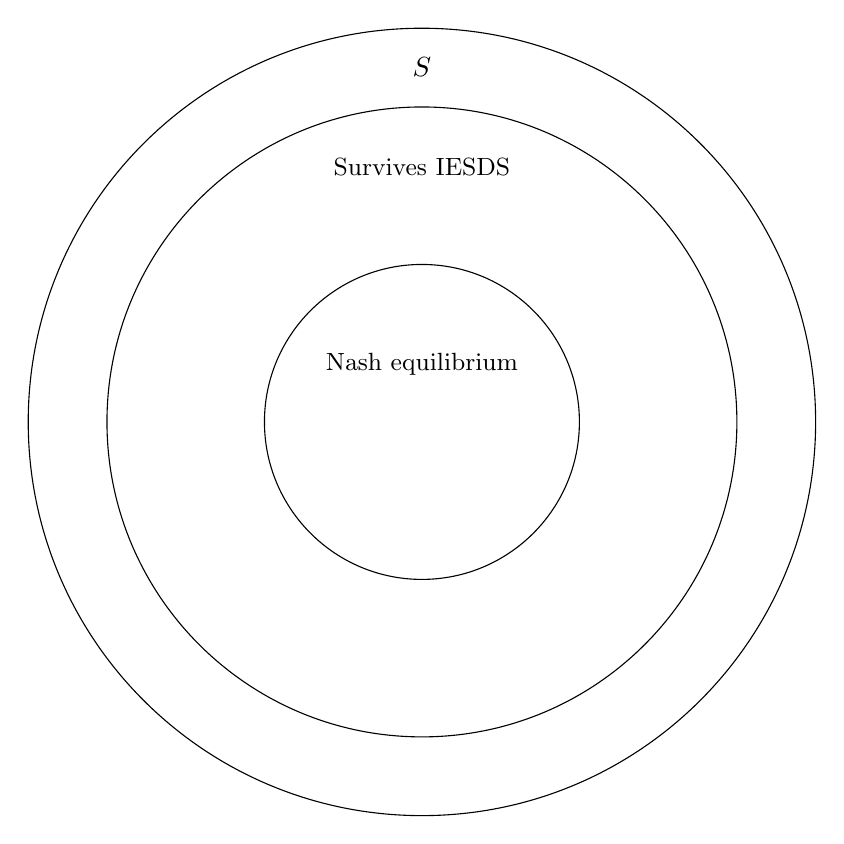
\begin{tikzpicture}
        \draw (0,0) circle (5cm);
        \draw (0,0) circle (4cm);
        \draw (0,0) circle (2cm);
        \node[anchor = north] at (0,4.75) {$S$};
        \node[anchor = south] at (0,3) {\small Survives IESDS};
        \node[anchor = north] at (0,1) {\small Nash equilibrium};
      \end{tikzpicture}
    \end{center}
  \end{problem}
  \begin{problem}{Voter Participation and Nash Equilibrium Activity}
    \begin{tcbraster}[raster columns = 2,colframe = black!75!white,colback=white]
      \tcbincludepdf{images/activity_2.pdf}
    \end{tcbraster}
  \end{problem}
  \begin{problem}{Bertrand Competition}
    \begin{description}
      \item[Assumptions] We have the following:
        \begin{description}
          \item[Players] Homogenous good produced by $n>1$ firms (i.e., oil, soybeans)
          \item[Cost] The cost of producing $q_i$ units to $c_i(q_i)$.
          \item[Demand] Total Market Demand is given by $D(p)$
          \item[Strategy Set] $S_i = \mathbb{R}^+$, where $p_i\in S_i$ denotes the price.
        \end{description}
      \item[Normal-Form Game] We have the following:
        \begin{description}
          \item[Players] $n=2$
          \item[Cost Function] $c_i(q_i) = cq_i$ for some $c\in \mathbb{R}^+$ and for $i=1,2$
          \item[Payoffs] $v_i(p_i,p_j) = \begin{cases}
              0, & p_i>p_j\\
              (p_i-c)(D(p_i)), & p_i<p_j\\
              \frac{1}{2}(p_i-c)(D(p_i)), & p_i=p_j
            \end{cases}$
        \end{description}
    \end{description}
  \end{problem}
  \begin{problem}{Bertrand Duopoly}
    \begin{tcbraster}[raster columns = 2,colframe = black!75!white,colback=white]
      \tcbincludepdf{images/activity_3.pdf}
    \end{tcbraster}
  \end{problem}
  \begin{problem}{Best Response Correspondence and finding Nash Equilibria}
    \begin{itemize}
      \item To find a Nash Equilibrium, it is helpful to determine which actions are best for a player given the actions of their opponents.
      \item A \textit{best response correspondence} is:
        \[
          BR_i(s_{-i}) = \{s_i\in S\mid v_i(s_i,s_{-i}) \geq v_i(s_i', s_{-i})~\forall s_i'\in S_i\}
        \] 
      \item Any strategy in $BR_i(s_{-i})$ is at least as good for player $i$ as every other strategy available to player $i$ when the other players' strategies are given by $s_{-i}$.
      \item We call it a correspondence, as oppposed to a function, since $BR_i(s_i)$ can be set-valued
    \end{itemize}
    A strategy profile $s^*$ is a Nash Equilibrium of $G$ if and only if every player's strategy is a best response to the other players' strategies:
    \[
      s^* \in BR_i(s^*_i)~\forall i
    \] 
    Essentially, every player is playing their best response given that everyone else is also playing their best response.\\

    There are two primary ways to find a Pure Strategy Nash Equilibrium:
    \begin{itemize}
      \item Refining educated guesses (e.g., Bertrand competition), necessary when best responses are set-valued
      \item Intersection of best responses (e.g., Payoff Matrix, Cournot competition)
    \end{itemize}
  \end{problem}
  \begin{problem}{Calculus and Best Response}
    In many cases, $BR_i(s_{-i})$ is a solution to the following problem:
    \[
      \max_{s_i}v_i(s_i,s_{-i})
    \] 
    Essentially, we have to solve an optimization problem: find the value of $s_i$ such that $v_i(s_i,s_{-i})$ is maximized.\\

    Consider the following payoff function:
    \[
      v_1(x_1,x_2) = 3x_1x_2 - x_1^2
    \] 
    We must use partial derivatives (as we're holding the strategy of $x_2$ constant in order to find the best response):
    \begin{align*}
      0 &= \frac{\partial v_1}{\partial x_1}\\
        &= 3x_2 - 2x_1\\
      x_1 &= \frac{3x_2}{2}
    \end{align*}
    Therefore, $BR_1(x_2) = x_1 = \frac{3x_2}{2}$.\\

    In order to find the Nash Equilibrium, we have to find the best response function for every player and take the intersections of all the best response functions.
  \end{problem}
  \begin{problem}{Cournot Competition}
    \begin{itemize}
      \item $n$ firms.
      \item Selling a homogenous identical good.
      \item \textit{Quantity} Competition: $S_i = \mathbb{R}^+$
      \item Payoff function:
        \[
          v_i(q_i,q_{-i}) = q_i P\left(\sum_{j = 1}^{n} q_j\right) - c(q_i)
        \] 
        What makes Cournot competition a game is that the payoff depends on the strategies of other players.
    \end{itemize}
  \end{problem}
  \begin{problem}{Cournot Duopoly: Example}
    \begin{itemize}
      \item $n=2$, $c(q_i) = 10q_i~\forall i$
      \item $P(Q) = \begin{cases}100-Q,&Q\leq 100\\0,&Q>100\end{cases}$
    \end{itemize}
    Three steps to find Nash Equilibrium:
    \begin{enumerate}[(i)]
      \item $BR_1(q_2)$
      \item $BR_2(q_1)$
      \item $(q_1^*,q_2^*)$ is a Nash Equilibrium where $q_1^* = BR_1(BR_2(q_1^*))$ (this follows from the definition of a Nash Equilibrium).
    \end{enumerate}
    \begin{align*}
      \max_{q_1} q_1(100-q_1-q_2)-10q_1 &= \max_{q_1} q_1(90-q_1-q_2)\\
      0 &= \frac{\partial v_1}{\partial q_1}\\
        &= 90-q_2-2q_1\\
      q_1 &= 45-\frac{1}{2}q_2
    \end{align*}
    \begin{align*}
      \max_{q_2} q_2(100-q_2-q_1)-10q_2 &= \max_{q_2}q_2(90-q_1-q_2)\\
      0&=\frac{\partial v_2}{q_2}\\
       &= 90-q_1-2q_2\\
      q_2 &= \frac{90-q_1}{2}
    \end{align*}
    \begin{description}
      \small
      \item[Note] In a symmetric game, every player's best response is identical with respect to every other player. You can only use this shortcut \textit{after} finding the best response.
    \end{description}
    \begin{align*}
      q_1^{*} &= BR_1(BR_2(q_1^*))\\
              &= \frac{90-\frac{90-q_1^*}{2}}{2}\\
              &= \frac{45}{2}+\frac{q_1^*}{4}\\
      q_1^* &= 30\\
      q_2^* &= BR(30)\\
            &= 30
    \end{align*}
    \begin{description}
      \small
      \item[Note] In a symmetric game, $q_1^* = q_2^*$, and similar for the $n$ player case.
    \end{description}
  \end{problem}
  \begin{problem}{Cournot Duopoly Variations}
    \begin{tcbraster}[raster columns = 2,colframe = black!75!white,colback=white]
      \tcbincludepdf{images/activity_4.pdf}
    \end{tcbraster}
  \end{problem}
  \begin{problem}{Mixed Strategies}
    \begin{center}
      \renewcommand{\arraystretch}{1.5}
      \begin{tabular}{cc|c|c|}
        \multicolumn{1}{c}{}&\multicolumn{1}{c}{}&\multicolumn{2}{c}{IRS}\\
                            &\multicolumn{1}{c}{}&\multicolumn{1}{c}{Audit ($A$)} & \multicolumn{1}{c}{Don't ($D$)}\\
        \cline{3-4}
        \multirow{2}{4em}{Taxpayer} & Honest ($H$) & $10,9$ & $10,10$ \\
        \cline{3-4}
                                    & Cheat ($C$) & $-35,10$ & $15,5$\\
        \cline{3-4}
      \end{tabular}
    \end{center}
    In a game like Rochambeau or the Tax Audit game (above), there is no pure strategy Nash equilibrium (i.e., there is always some incentive to deviate regardless of the outcome). Many other games, especially in the realms of sports and the military, feature a lack of pure strategy Nash equilibria.\\

    Players must randomize over the possible strategy spaces to maximize their payoff, rather than depending on a pure strategy.
    \begin{itemize}
      \item A \textit{mixed strategy}, $\sigma_i$, of player $i$ is a probability distribution over $S_i$.
      \item There are two primary properties of a probability distribution:
        \begin{itemize}
          \item $\sigma_i(s_i) \geq 0$ for all $s_i \in S_i$ (something cannot have negative probability).
          \item $\sum_{s_i\in S_i}\sigma_i(s_i) = 1$ (everything must happen).
        \end{itemize}
      \item There are multiple ways to write the mixed strategy:
        \begin{itemize}
          \item Functions: $\sigma_1(H) = 1/3$, $\sigma_1(T) = 2/3$
          \item Vector: $\sigma_1 = \langle 1/3,2/3\rangle$
          \item Type $2$ Vector: $\sigma_1 = \frac{1}{3}H + \frac{2}{3}T$
        \end{itemize}
    \end{itemize}
  \end{problem}
  \begin{problem}{Mixed Strategy Profiles and Expected Payoffs}
    A mixed strategy profile $\sigma = (\sigma_1,\sigma_2,\dots,\sigma_n)$ is a set of mixed strategies in the game.\\

    The expected payoff to player $i$ with the mixed strategy profile $(\sigma_i, \sigma_{-i})$ is as follows:
    \[
      v_i(\sigma_i,\sigma_{-i}) = \sum_{s_i\in S_i}\sum_{s_{-i}\in S_{-i}}\sigma_i(s_i)\sigma_{-i}(s_{-i})v_i(s_i,s_{-i})
    \] 
    \begin{description}
      \item[Note:] This is equivalent to the weighted average of the payoffs of the pure strategy profiles.
    \end{description}
    For example, in the tax game, let $\sigma_1 = \frac{3}{4}H + \frac{1}{4}C$ and $\sigma_2 = \frac{1}{3}A + \frac{2}{3}D$. Then, we have the total payoff as follows:
    \begin{align*}
      v_1(\sigma_1,\sigma_2) &= \frac{3}{4}\frac{1}{3}(10) + \frac{3}{4}\frac{2}{3}(10) + \frac{1}{4}\frac{1}{3}(-35) + \frac{1}{4}\frac{2}{3}(15)\\
                             &= \frac{85}{12}
    \end{align*}
    Therefore, $\frac{85}{12}$ is the \textit{expected payoff}.
  \end{problem}
  \begin{problem}{Mixed Strategy Nash Equilibrium}
    Let $\sigma^*$ be a mixed strategy profile. Then, if
    \[
      v_i(\sigma^*_i,\sigma^*_{-i}) \geq v_i(\sigma_i,\sigma^*_{-i})
    \] 
    for all players $i$ and all mixed strategies $\sigma_i$, $\sigma^*_i$ is the \textit{mixed strategy Nash equilibrium}.\\

    Instead of checking all mixed strategies, we only need check if switching to any \textit{pure} strategy makes a player better off. If it is not, the mixed strategy profile is a Nash equilibrium.
    \[
      v_i(\sigma^*_i,\sigma^*_{-i}) \geq v_i(s_i,\sigma^*_{-i})~\forall s_i\in S_i
    \] 
    Many mixed strategy Nash equilibria are not strict Nash equilibria (i.e., there are other strategies with similar payoffs).
  \end{problem}
  \begin{problem}{Finding Mixed Strategy Nash Equilibria}
    In a finite game, the \textit{support} of a mixed strategy $\sigma_i$, $\text{supp}(\sigma_i)$ is the set of strategies to which $\sigma_i$ has strictly positive probability:
    \[
      \text{supp}(\sigma_i) = \{s_i\in S_i \mid \sigma_i(s_i) > 0\}
    \]
    If $\sigma^*$ is a mixed strategy Nash equilibrium, and $s_i',s_i'' \in \text{supp}(\sigma_i)$, then
    \[
      v_i(s_i',\sigma_i) = v_i(s_i'',\sigma_i)
    \] 
    Essentially, if a player is playing two strategies with positive probability, they have to be indifferent between the two strategies (or else they would play the one with a higher payoff).
  \end{problem}
  \begin{problem}{Mixed Strategy Nash Equilibrium Example}
    \begin{center}
      \renewcommand{\arraystretch}{1.5}
      \begin{tabular}{cc|c|c|}
        \multicolumn{1}{c}{}&\multicolumn{1}{c}{}&\multicolumn{2}{c}{IRS}\\
                            &\multicolumn{1}{c}{}&\multicolumn{1}{c}{Audit ($A$)} & \multicolumn{1}{c}{Don't ($D$)}\\
        \cline{3-4}
        \multirow{2}{4em}{Taxpayer} & Honest ($H$) & $10,9$ & $10,10$ \\
        \cline{3-4}
                                    & Cheat ($C$) & $-35,10$ & $15,5$\\
        \cline{3-4}
      \end{tabular}
    \end{center}
    \begin{align*}
      \sigma_1 &= pH + (1-p) C\\
      \sigma_1 &= qA + (1-q) D
    \end{align*}
    Player 1's Indifference:
    \begin{align*}
      v_1(H,\sigma_2) &= 10\\
      v_2(C,\sigma_2) &= -35q + 15(1-q)\\
      10 &= 15-50q\tag*{when taxpayer will be indifferent}\\
      q^* &= \frac{1}{10}
    \end{align*}
    Player 2's Indifference:
    \begin{align*}
      v_2(\sigma_1,A) &= 9p + 10(1-p)\\
      v_2(\sigma_1,D) &= 10p + 5(1-p)\\
      10-p &= 5+5p \\
      p^* &= \frac{5}{6}
    \end{align*}
    The Nash equilibrium is where $p^* = 5/6$ and $q^* = 1/10$.
  \end{problem}
  \begin{problem}{Mixed Strategy Nash Equilibrium: D-Day}
    \begin{tcbraster}[raster columns = 1,colframe = black!75!white,colback=white]
      \tcbincludepdf{images/activity_5.pdf}
    \end{tcbraster}
  \end{problem}
  \begin{problem}{Finding Mixed Strategy Nash Equilibria in Larger Games}
    In the $2\times 2$ games, we did not have to worry about which strategies were in the support of the strategies played in Nash equilibrium, but we do in higher dimensional games.
    \begin{center}
      \renewcommand{\arraystretch}{1.5}
      \begin{tabular}{c|c|c|c|}
        \multicolumn{1}{c}{} & \multicolumn{1}{c}{$L$} & \multicolumn{1}{c}{$C$} & \multicolumn{1}{c}{$R$}\\
        \cline{2-4}
        $U$ & $10,9$ & $10,6$ & $10,10$ \\
        \cline{2-4}
        $M$ & $-5,9$ & $15,10$ & $11,12$\\
        \cline{2-4}
        $D$ & $-35,10$ & $10,7$ & $15,5$\\
        \cline{2-4}
      \end{tabular}
    \end{center}
  \end{problem}
  \begin{problem}{Reducing Size of Larger Games}
    A strategy $s_i'$ is \textit{strictly dominated} if there exists a mixed strategy $\sigma_i$ such that
    \[
      v_i(\sigma_i,s_{-i}) > v_i(s_i',s_{-i})
    \] 
    for every $s_{-i}\in S_{-i}$.\\

    Essentially, if we can find a mixed strategy profile that is strictly better than the pure strategy, the pure strategy is strictly dominated.\\

    In the previous game, we can use IESDS as follows:
    \begin{itemize}
      \item No strategies are strictly dominated by pure strategies.
      \item However, $C$ is strictly dominated by $\frac{1}{2}L + \frac{1}{2}R$
    \end{itemize}
    \begin{center}
      \renewcommand{\arraystretch}{1.5}
      \begin{tabular}{c|c|c|c|}
        \multicolumn{1}{c}{} & \multicolumn{1}{c}{$L$} & \multicolumn{1}{c}{$C$} & \multicolumn{1}{c}{$R$}\\
        \cline{2-4}
        $U$ & $10,9$ & $\xcancel{10,6}$ & $10,10$ \\
        \cline{2-4}
        $M$ & $-5,9$ & $\xcancel{15,10}$ & $11,12$\\
        \cline{2-4}
        $D$ & $-35,10$ & $\xcancel{10,7}$ & $15,5$\\
        \cline{2-4}
      \end{tabular}
    \end{center}
    \begin{itemize}
      \item Additionally, $M$ is strictly dominated by $\frac{3}{4}U + \frac{1}{4}D$
    \end{itemize}
    \begin{center}
      \renewcommand{\arraystretch}{1.5}
      \begin{tabular}{c|c|c|c|}
        \multicolumn{1}{c}{} & \multicolumn{1}{c}{$L$} & \multicolumn{1}{c}{$C$} & \multicolumn{1}{c}{$R$}\\
        \cline{2-4}
        $U$ & $10,9$ & $\xcancel{10,6}$ & $10,10$ \\
        \cline{2-4}
        $M$ & $\xcancel{-5,9}$ & $\xcancel{15,10}$ & $\xcancel{11,12}$\\
        \cline{2-4}
        $D$ & $-35,10$ & $\xcancel{10,7}$ & $15,5$\\
        \cline{2-4}
      \end{tabular}
    \end{center}
    Since, from here, we cannot find any strictly dominated strategies, we have to use our method for finding mixed strategy Nash equilibria.\\

    By using the method, we find that the solutions are $p = 5/6$ on $U$ and $q=1/10$ on $L$.
    \begin{description}
      \tiny
      \item[Note:] After IESDS, the game is the same as the Tax Audit Game from earlier.
    \end{description}
  \end{problem}
  \begin{problem}{Mixed Strategy Nash Equilibria in Larger Game Example}
    \begin{tcbraster}[raster columns = 2,colframe = black!75!white,colback=white]
      \tcbincludepdf{images/activity_6.pdf}
    \end{tcbraster}
  \end{problem}
  \begin{problem}{Multiple Equilibria}
    Meet in New York: you and your friend have agreed to meet in New York at 12pm. Both of your phones have died. Where do you go?\\

    There are multiple Nash equilibria to this game (essentially, basically anywhere).
  \end{problem}
  \begin{problem}{Interpreting Nash Equilibria}
    IESDS is a constructive process to \textit{predict} play in a game; it does not assume that players know the strategy choices of other players.\\

    In a Nash equilibrium, players have self-fulfilling beliefs about the play of others. Essentially, Nash equilibria survive IESDS, and then players respond to \textit{correct} beliefs.\\

    We might ask where the beliefs come from:
    \begin{description}
      \item[Play Prescription:] An outside party tells people how to play.
      \item[Pre-play Communication:] Players communicate and agree on how to play the game.
      \item[Rational Introspection:] A Nash equilibrium seems reasonable because my beliefs of what other players do are consistent with them being rational. This works in games with a unique Nash equilibrium.
      \item[Focal Point:] Social norms lead players to prefer certain actions over others.
      \item[Learning:] Players play many times, and learn what other people prioritize by doing so.
      \item[Evolution:] Players are programmed to play a certain action; if they do not play a Nash equilibrium, they ``mutate.'' If this deviation is profitable, the players will ``multiply'' at a faster rate than other players and eventually take over. This system converges to a state where all players choose the Nash equilibrium.
    \end{description}
  \end{problem}
  \begin{problem}{Existence of Nash Equilibria}
    The set of strategies played in Nash equilibrium is a subset of the strategies that survive IESDS. The Nash equilibrium isn't so strong such that there is no Nash equilibrium.

    \begin{description}
      \item[Nash Theorem:] Every finite normal-form game has a mixed strategy Nash equilibrium.
    \end{description}
    \begin{description}
      \tiny
      \item[Note:] Pure strategy profiles are mixed strategy profiles with a degenerate probability distribution.
    \end{description}
    \begin{problem}{Intuition}
      \begin{description}
        \item[Lemma:] A mixed strategy profile $\sigma^*$ is a Nash equilibrium if and only if it is a fixed point of the best response correspondence:
          \begin{align*}
            \sigma^* \in BR(\sigma^*)\\
            \shortintertext{where}
            BR(\sigma) &= BR(\sigma_{-1}) \times BR(\sigma_{-2})\times\cdots\times BR(\sigma_{-n})
          \end{align*}
          \textit{If the mixed strategy profile is that which is the best response for every player in the mixed strategy profile, then that has to be a Nash equilibrium.}
      \end{description}
      In one dimension, we know that every continuous function $f: [a,b] \rightarrow [a,b]$ must have a fixed point (by the Intermediate Value Theorem).\\

      In $\mathbb{R}^n$, a continuous function from a compact (i.e., bounded and closed), convex (i.e., every two points in the set can be connected by a line) subset to itself must also have a fixed point (by Brouwer's Fixed Point Theorem).\\

      Then, Shizuo Kakutani proved that Brouwer's result applied to particular types of correspondences.\\

      A correspondence $r: X\rightarrow X$ has a fixed point such that $x\in r(x)$ if:
      \begin{itemize}
        \item $X$ is a compact, convex, non-empty subset of $\mathbb{R}^n$
        \item $r(x)$ is nonempty for all $x$.
        \item $r(x)$ is convex for all $x$.
        \item $r$ has a closed graph.
      \end{itemize}
      Nash showed that the best response correspondence satisfied these conditions.
    \end{problem}
  \end{problem}
  \begin{problem}{Generic Properties}
    A property is \textit{generic} if, given the number of players and strategies, the property is true with probability $1$ for payoffs chosen at random.\\

    For example, the property ``In a Nash equilibrium players $1$ and $2$ obtain different payoffs'' is generic (i.e., if you throw in random payoffs, players will almost certainly have different payoffs).\\

    Additionally, the property ``A finite strategic game has a finite and odd number of Nash equilibria.'' is generic.
    \begin{itemize}
      \item When looking for (mixed strategy) Nash equilibria, if you find an even number, you probably missed one.
    \end{itemize}
  \end{problem}
  \section*{Sequential Games of Complete Information}%
  
  \begin{problem}{Extensive Form Games}
    Consider a variant of the Matching Pennies in which Player 2 observes the choice made by Player 1 before making their choice.
    \begin{center}
      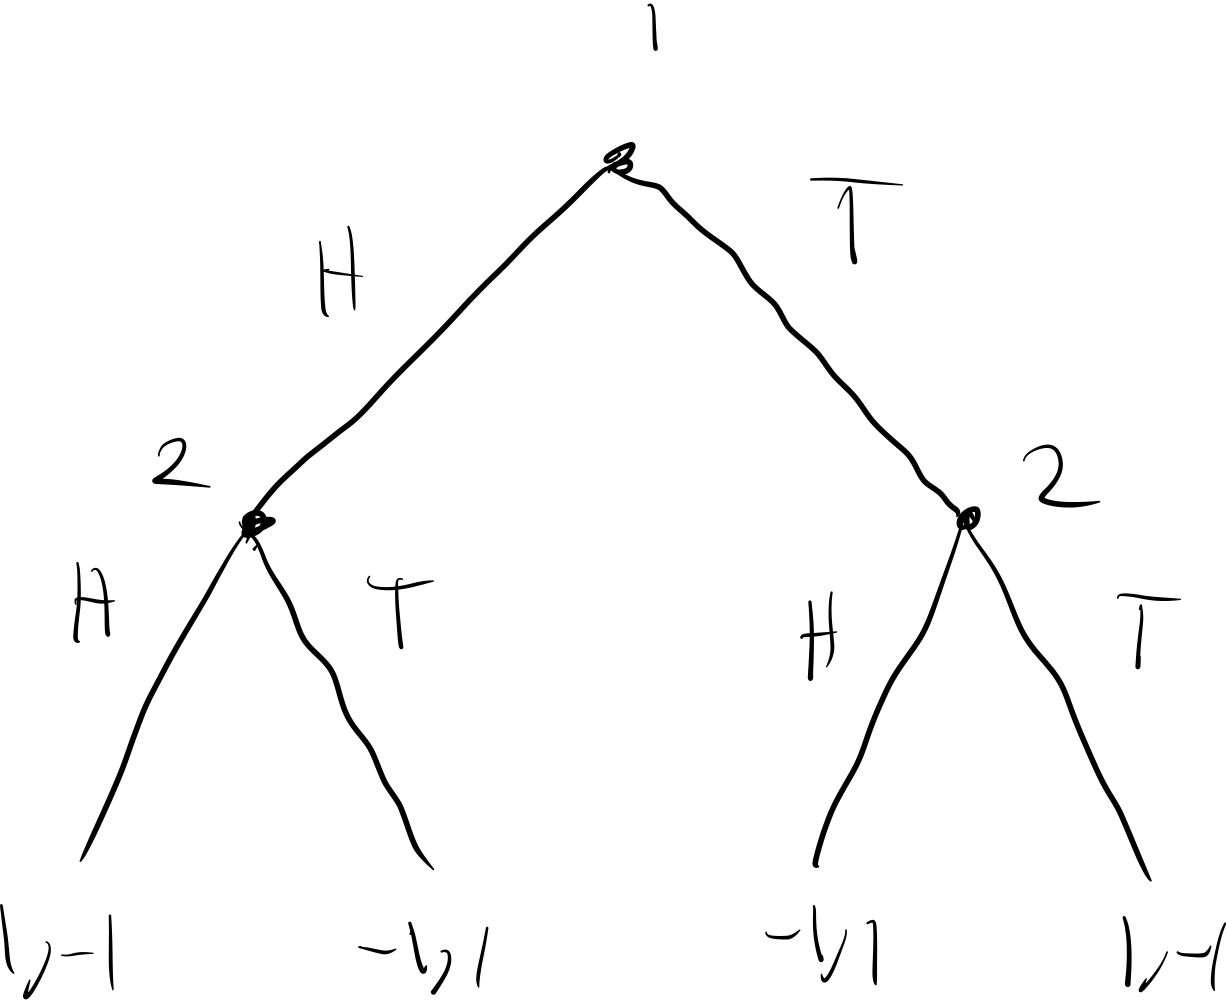
\includegraphics[width=7cm]{images/matching_pennies_tree.png}
    \end{center}
    We can model the simultaneous move version by connecting the Player 2 nodes with a dashed line.
    \begin{center}
      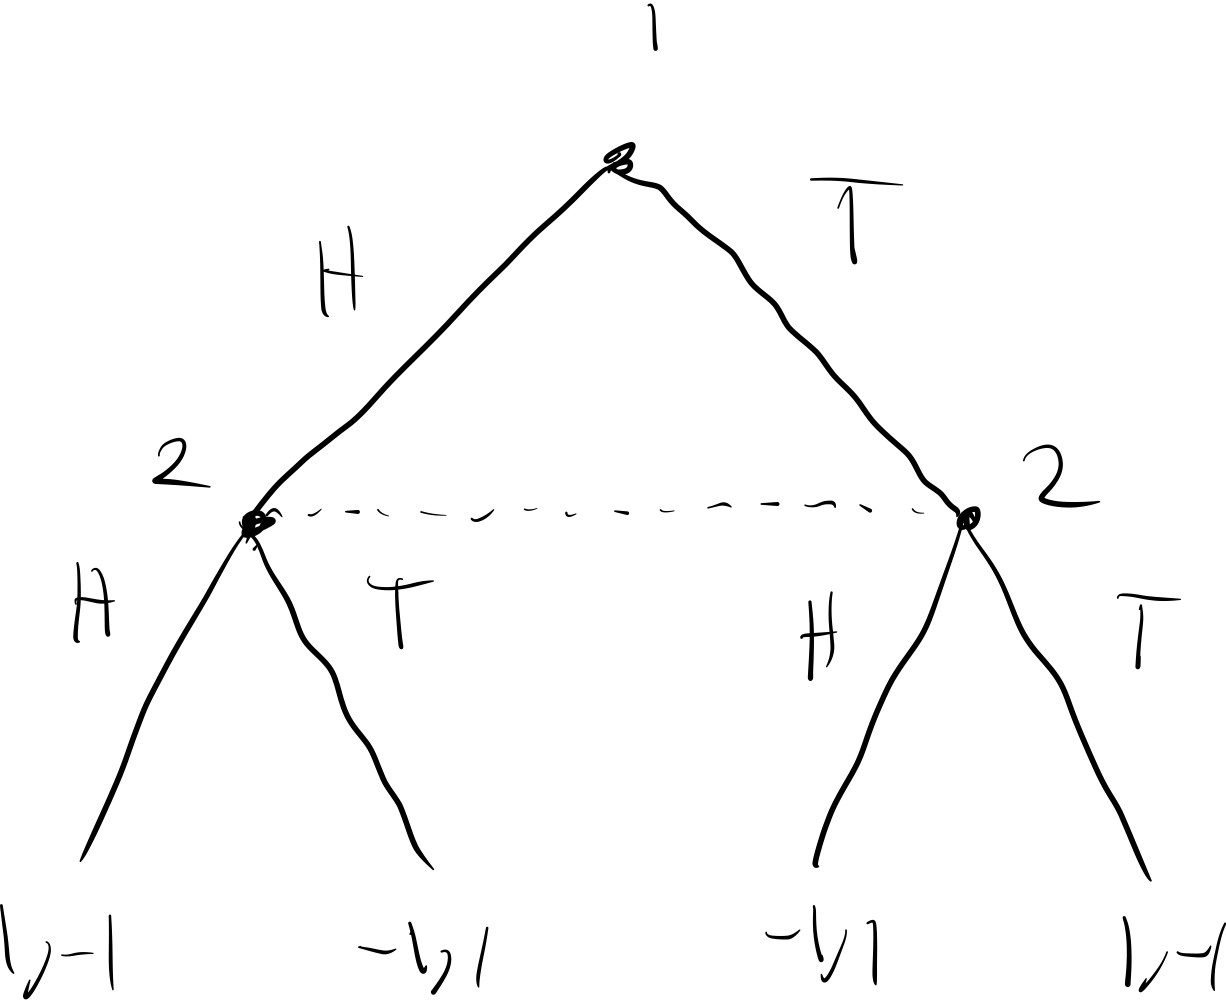
\includegraphics[width=7cm]{images/matching_pennies_simultaneous.png}
    \end{center}
    \begin{description}
      \item[Definition] A \textit{finite horizon extensive form game} consists of
        \begin{enumerate}[(1)]
          \item The set of players
          \item A set of \textit{decision nodes} where at each node it is specified:
            \begin{enumerate}[(i)]
              \item the player who moves
              \item the set of possible actions
              \item the successor node resulting from each action
            \end{enumerate}
          \item Payoffs upon reaching a \textit{terminal node}
          \item What each player knows at each of the decision nodes, described by a collection of \textit{information sets} that partition the set of decision nodes.
        \end{enumerate}
      \item[Definition] A \textit{information set} is a collection of decision nodes such that at every node in the set:
        \begin{enumerate}[(i)]
          \item The same player has the move
          \item The same set of possible actions is available.
        \end{enumerate}
        When the play of the game reaches a node in the information set, the player with the move does not know which node in the information set has or has not been reached.\newline

        A player can have multiple information sets, but each node must be in an information set.
    \end{description}
  \end{problem}
  \begin{problem}{Perfect Information}
    A game of perfect information is a game in which all the information sets are singletons (but a player can have multiple information sets):
    \begin{itemize}
      \item In a game of perfect information, a player knows every move made by players before them.
      \item Sequential Matching Pennies is a game of perfect information, but Matching Pennies is a game of imperfect information.
      \item All normal form games can be thought of as extensive games with imperfect information.
    \end{itemize}
  \end{problem}
  \begin{problem}{Pure Strategies in Extensive Form Games}
    A pure strategy for a player in an extensive form game is a complete set of contingent actions (even if they are never played or never able to be played) for each player at each information set. In the sequential Matching Pennies, we label each contingency:
    \begin{center}
      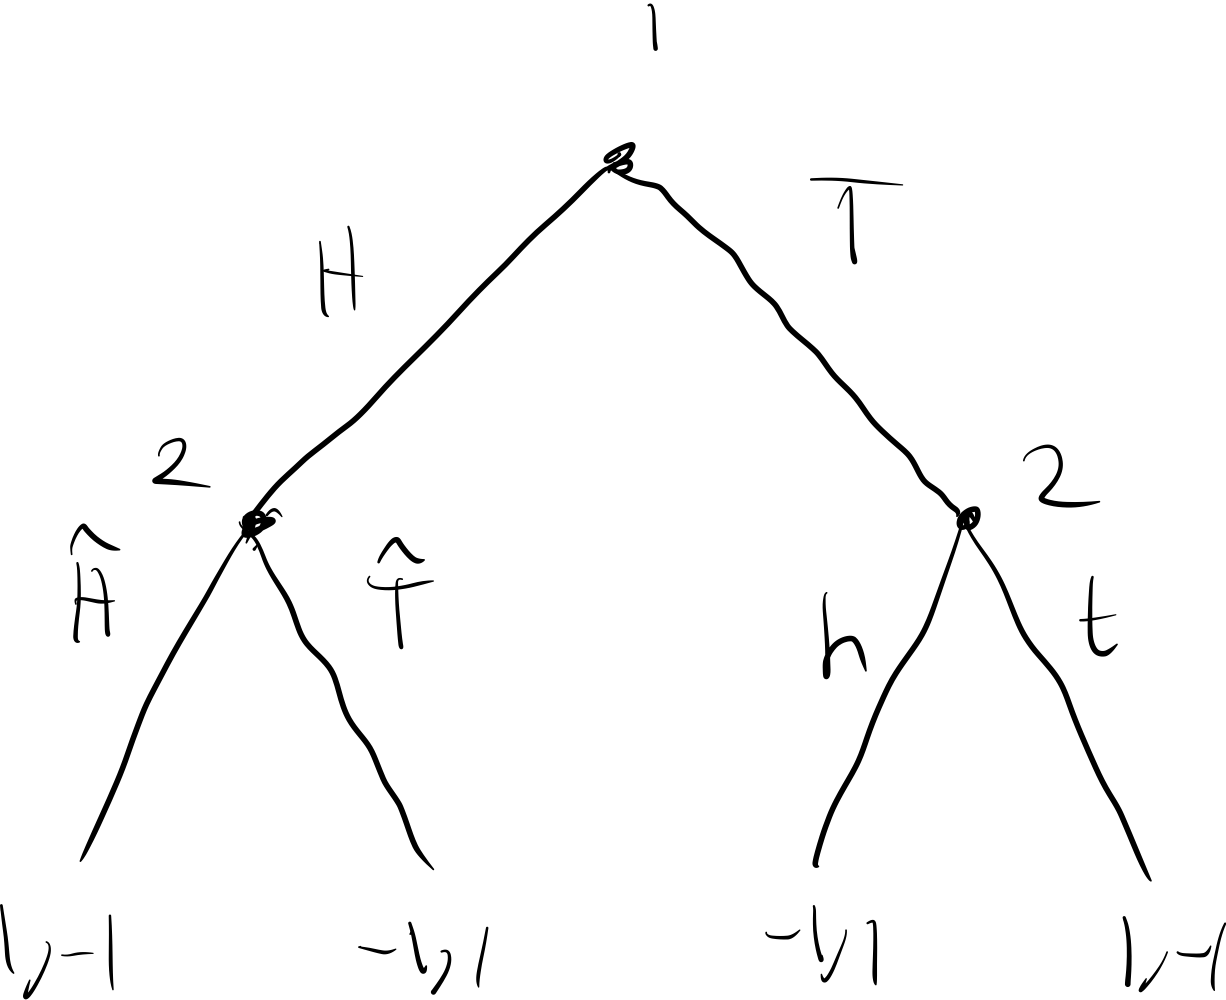
\includegraphics[width=7cm]{images/matching_pennies_pure_strategies.png}
    \end{center}
    Then, we can create the normal form game as follows:
    \begin{center}
      \renewcommand{\arraystretch}{1.5}
      \begin{tabular}{c|c|c|c|c|}
        \multicolumn{1}{c}{}& \multicolumn{1}{c}{$\hat{H}h$} & \multicolumn{1}{c}{$\hat{H}t$} & \multicolumn{1}{c}{$\hat{T}h$} & \multicolumn{1}{c}{$\hat{T}t$}\\
        \cline{2-5}
        $H$ & $1,-1$ & $1,-1$ & $-1,1$ & $-1,1$\\
        \cline{2-5}
        $T$ & $-1,1$ & $1,-1$ & $-1,1$ & $1,-1$\\
        \cline{2-5}
      \end{tabular}
    \end{center}
    where we denote Player 2's strategies by $xy$, where $x = s_2(H)$ and $y = s_2(T)$.\newline

    The Entry game (in Industrial Organization) has the following extensive form:
    \begin{center}
      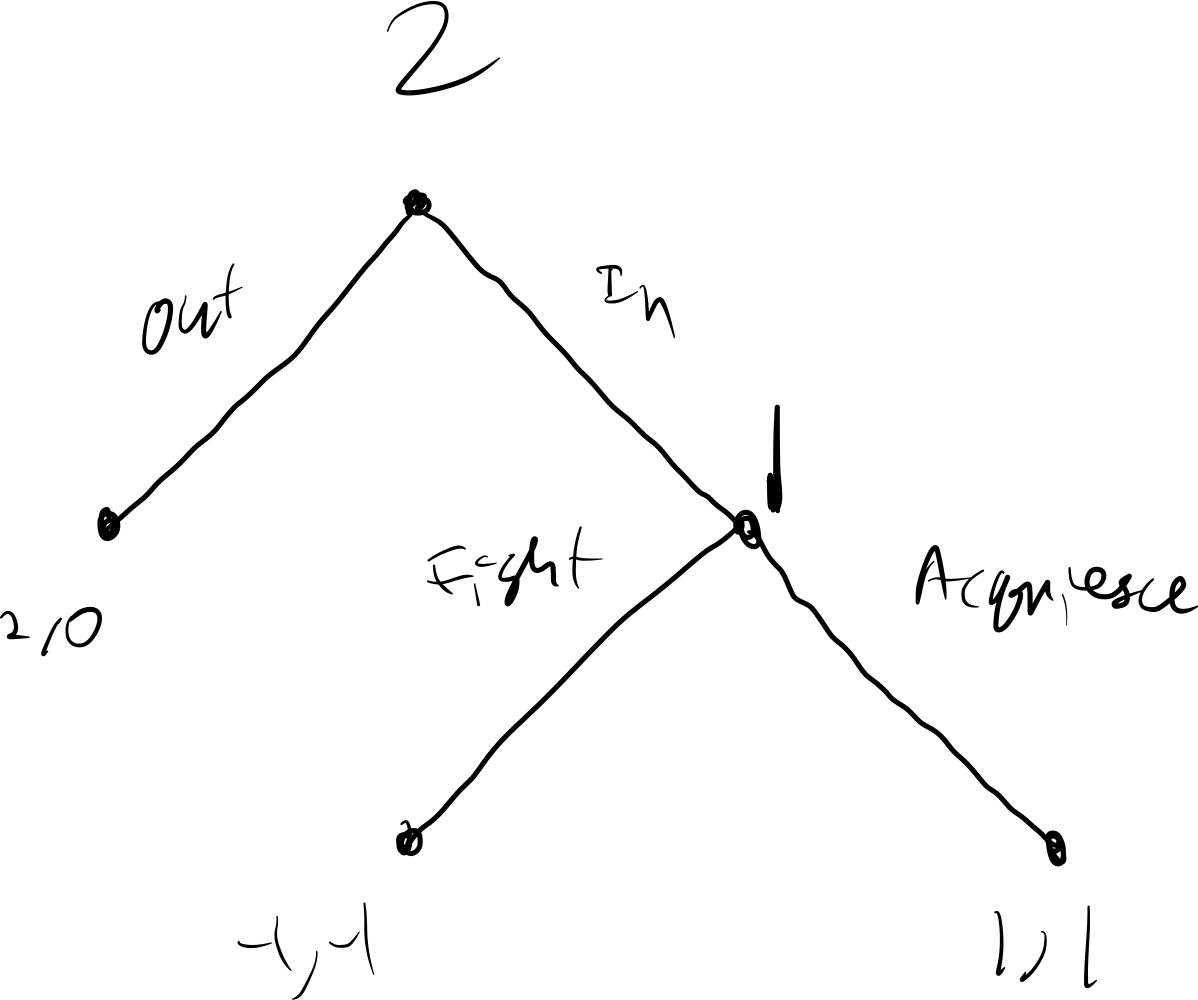
\includegraphics[width=7cm]{images/entry_extensive.png}
    \end{center}
    and the normal form game is as follows:
    \begin{center}
      \renewcommand{\arraystretch}{1.5}
      \begin{tabular}{c|c|c|}
        \multicolumn{1}{c}{} & \multicolumn{1}{c}{Out} & \multicolumn{1}{c}{In}\\
        \cline{2-3}
        Fight & $2,0$ & $-1,-1$\\
        \cline{2-3}
        Acquiesce & $2,0$ & $1,1$\\
        \cline{2-3}
      \end{tabular}
    \end{center}
    Notice that Player 1 still has to include the payoffs for Fight and Acquiesce \textit{even if Player 2 plays Out.}
  \end{problem}
  \begin{problem}{Behavioral Strategies}
    A behavioral strategy for player $i$ is a function that assigns a probability distribution over the actions available to player $i$ at each information set where player $i$ moves.\newline
    
    This is different from a mixed strategy since a mixed strategy is a mixture over all the pure strategies, rather than a mixture at each action.\newline

    Given perfect recall, the mixed strategy profile can be created by multiplying the behavioral strategies together.
  \end{problem}
  \begin{problem}{Extensive Form Games Example}
    \begin{tcbraster}[raster columns = 2,colframe = black!75!white,colback=white]
      \tcbincludepdf{images/activity_7.pdf}
    \end{tcbraster}
  \end{problem}
  \begin{problem}{Equilibrium in Extensive Form Games}
    \begin{itemize}
      \item A Nash equilibrium is still a strategy profile in which no player has a unilateral profitable deviation.
      \item The Nash Equilibrium of an extensive form game are the Nash equilibria of the game's normal form representation.
      \item We can apply the methods from the first third of the course to find the Nash equilibrium.
    \end{itemize}
    In the entry game, we have the following normal form:
    \begin{center}
      \renewcommand{\arraystretch}{1.5}
      \begin{tabular}{c|c|c|}
        \multicolumn{1}{c}{} & \multicolumn{1}{c}{Out} & \multicolumn{1}{c}{In}\\
        \cline{2-3}
        Fight & $2,0$ & $-1,-1$\\
        \cline{2-3}
        Acquiesce & $2,0$ & $1,1$\\
        \cline{2-3}
      \end{tabular}
    \end{center}
    There are an infinite number of Nash equilibria:
    \begin{itemize}
      \item $(F,O)$: the challenger will stay out if it thinks the incumbent will fight; however, the challenger can call Firm 1's bluff and enter the market.
      \item $(A,I)$: if the challenger enters the market, Firm 1 will acquiesce.
      \item $(pF + (1-p)A, O)$ for $p \geq 1/2$: Firm 1 needs to mix between fight and acquiesce such that Firm 2 stays out.
    \end{itemize}
    Given the fact that $(F,O)$ is not a credible threat, we need a better concept for equilibrium that rules out non-credible threats.\newline

    For another example of a non-credible threat, consider Stackelberg Competition:
    \begin{itemize}
      \item Firm 1 chooses $q_1 \in [0,1]$
      \item Firm 2 sees $q_1$, then chooses $q_2\in[0,1]$
      \item Let $c_1(q_1) = c_2(q_2) = 0$, and $P(q_1,q_2) = 1-q_1-q_2$
      \item We claim that for any $q_1' = [0,1]$, the game has a Nash equilibrium in which firm 1 produces $q_1'$.
        \begin{align*}
          s_2(q_1) &= \begin{cases}
            \frac{1-q_1'}{2}&q_1=q_1'\\
            1-q_1 & q_1\neq q_1'
          \end{cases}
        \end{align*}
        \begin{description}
          \small
          \item[Note:] The Nash equilibrium must be one for the game's strategy profile.
        \end{description}
        \begin{itemize}
          \item If firm $1$ plays $q_1'$, then player $2$ plays its best response (anything off the equilibrium path).
          \item Given firm 2's strategy, firm $1$ makes positive profit by playing $q_1'$, or else firm $2$ floods the market, pushing the price to zero and yielding zero profits.
          \item This is a Nash equilibrium --- however, the second part of this statement is non-credible.
        \end{itemize}
    \end{itemize}
  \end{problem}
  \begin{problem}{Subgame Perfect Equilibrium}
    A \textbf{subgame} of an extensive form game has the following properties:
    \begin{itemize}
      \item Begins at a decision node $n$ that is a singleton information set.
      \item Includes \textit{all} the decision and terminal nodes following $n$ in the game tree.
      \item Does not ``cut through'' any information sets (drawing a circle around the subgame doesn't cut a dashed line)
    \end{itemize}
    The game is always a subgame of itself.\\

    A strategy profile $s^*$ is a \textit{subgame perfect equilibrium} if it is a Nash equilibrium of every subgame. It's important to remember that the payoffs in equilibrium are \textit{not} a SPE; only the strategy profile.
    \begin{itemize}
      \item Every SPE is a Nash equilibrium because the game is a subgame of itself.
      \item SPE is a refinement of Nash equilibrium because it is a subset of the set of Nash equilibria.
    \end{itemize}
    \begin{center}
      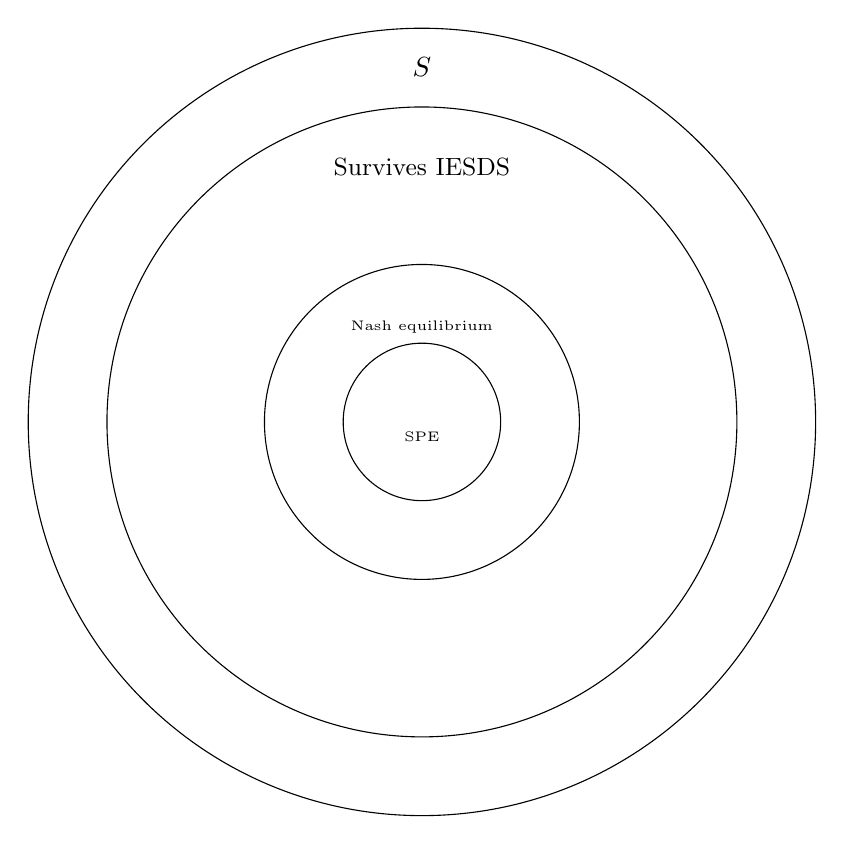
\begin{tikzpicture}
        \draw (0,0) circle (5cm);
        \draw (0,0) circle (4cm);
        \draw (0,0) circle (2cm);
        \draw (0,0) circle (1cm);
        \node[anchor = north] at (0,4.75) {$S$};
        \node[anchor = south] at (0,3) {\small Survives IESDS};
        \node[anchor = south] at (0,1) {\tiny Nash equilibrium};
        \node[anchor = north] at (0,0) {\tiny SPE};
      \end{tikzpicture}
    \end{center}
    In the Entry game, for example, there are an infinite number of Nash equilibria, but there is only one SPE: $(A,I)$, as it is the Nash equilibrium of the subgame starting from the ``in'' node.\\

    In Stackelberg Competition, we claim that the unique $SPE$ is $s_1^* = \frac{1}{2}$ and $s_2^*(q_1) = \frac{1-q_1}{2}$.
    \begin{description}
      \small
      \item[Note:] It would be wrong to write the proposed SPE as $(s_1^*,s_2^*) = (1/2,1/4)$, even though this is the outcome along the equilibrium path. Recall that a strategy is a complete contingent plan --- player 2's strategy has to be contingent on what player 1 does.
    \end{description}
    The subgames of Stackelberg competition are the game itself and the proper subgame that follows each possible choice of $q_1$. In each proper subgame, we have a $1$-player game, so the Nash equilibrium is equivalent to maximizing profit.
    \begin{align*}
      s_2^*(q_1) &= \max_{q_2}q_2(1-q_1-q_2)\\
                 &= \frac{1-q_1}{2}
    \end{align*}
    The Nash equilibrium of the entire game requires firm $1$ to best respond to firm $2$:
    \begin{align*}
      s_1^* &= \max_{q_1}q_1(1-q_1-s_2^*(q_1))\\
            &= 1/2
    \end{align*}
    \begin{description}
      \small
      \item[Note:] Firm 1 produces more than firm 2 and has higher profits --- this is emblematic of the first mover advantage. Firm 1 can find firm 2's best response function, then use that information to determine their own best response, as opposed to the Cournot game in which firm 1 and 2 have the same amount of information.
    \end{description}
  \end{problem}
  \begin{problem}{Backward Induction and Existence}
    The previous two examples show how to do \textit{backward induction}, in which we can solve finite extensive form games by starting at the subgames furthest down the game tree and moving backwards, finding the Nash equilibria in each subgame.\newline
    
    Every \textit{finite} (finite number of terminal nodes) extensive form game of perfect information has a \textit{pure strategy} SPE; generically, this SPE is unique.
    \begin{itemize}
      \item You solve the last rounds of the game, then replace these subgames with the outcome of the Nash equilibrium, and repeat the procedure.
    \end{itemize}
    Every finite extensive form game (not necessarily of perfect information) has a SPE.
    \begin{itemize}
      \item The refinement of Nash equilibrium is not too strong in the sense that a SPE always exists.
      \item Each subgame has a Nash equilibrium due to the Nash existence result.
    \end{itemize}
  \end{problem}
  \begin{problem}{Subgame Perfect Equilibria }
    \begin{tcbraster}[raster columns = 2,colframe = black!75!white,colback=white]
      \tcbincludepdf{images/activity_8.pdf}
    \end{tcbraster}
  \end{problem}
    \begin{problem}{Ultimatum Game}
      \begin{center}
        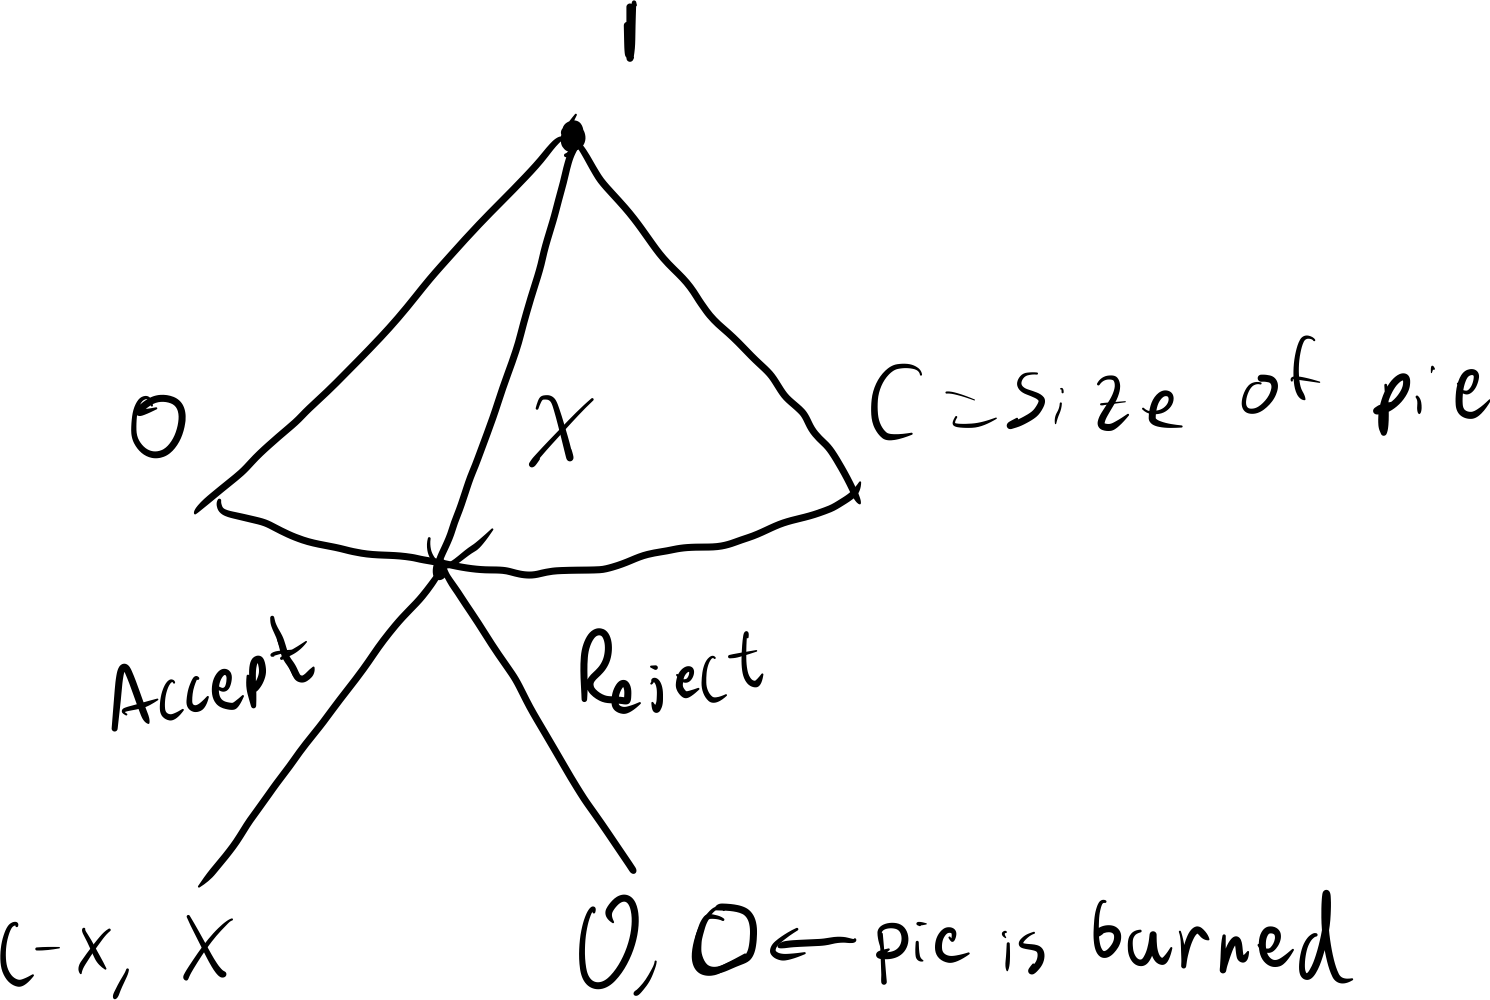
\includegraphics[width=10cm]{images/ultimatum.png}
      \end{center}
      \tcblower
      To find the subgame perfect equilibrium, we go as follows:
      \begin{itemize}
        \item Player 2: infinite information sets.
          \begin{itemize}
            \item Player 2 observes offer $x$.
            \item Player 2's best response:
              \begin{align*}
                s_2(x) &= \begin{cases}
                  A,&\text{if}~x>0\\
                  \alpha A + (1-\alpha)R,&\text{if}~x=0 \tag*{$\forall \alpha\in[0,1]$}
                \end{cases}
              \end{align*}
          \end{itemize}
        \item Player 1: 1 information set.
          \begin{itemize}
            \item Player 1's best response:
              \begin{align*}
                v_1(x,s_2(x)) &= \begin{cases}
                  c-x,&\text{if}~x>0\\
                  \alpha c,&\text{if}~x=0
                \end{cases}
              \end{align*}
            \item Player 1's best response \textit{only} exists if $\alpha = 1$.
          \end{itemize}
        \item Unique SPE:
          \begin{itemize}
            \item $s_1 = 0$
            \item $s_2(x) = A,~\forall x$
          \end{itemize}
      \end{itemize}
    \end{problem}
    \begin{problem}{Holdup Game}
      \begin{center}
        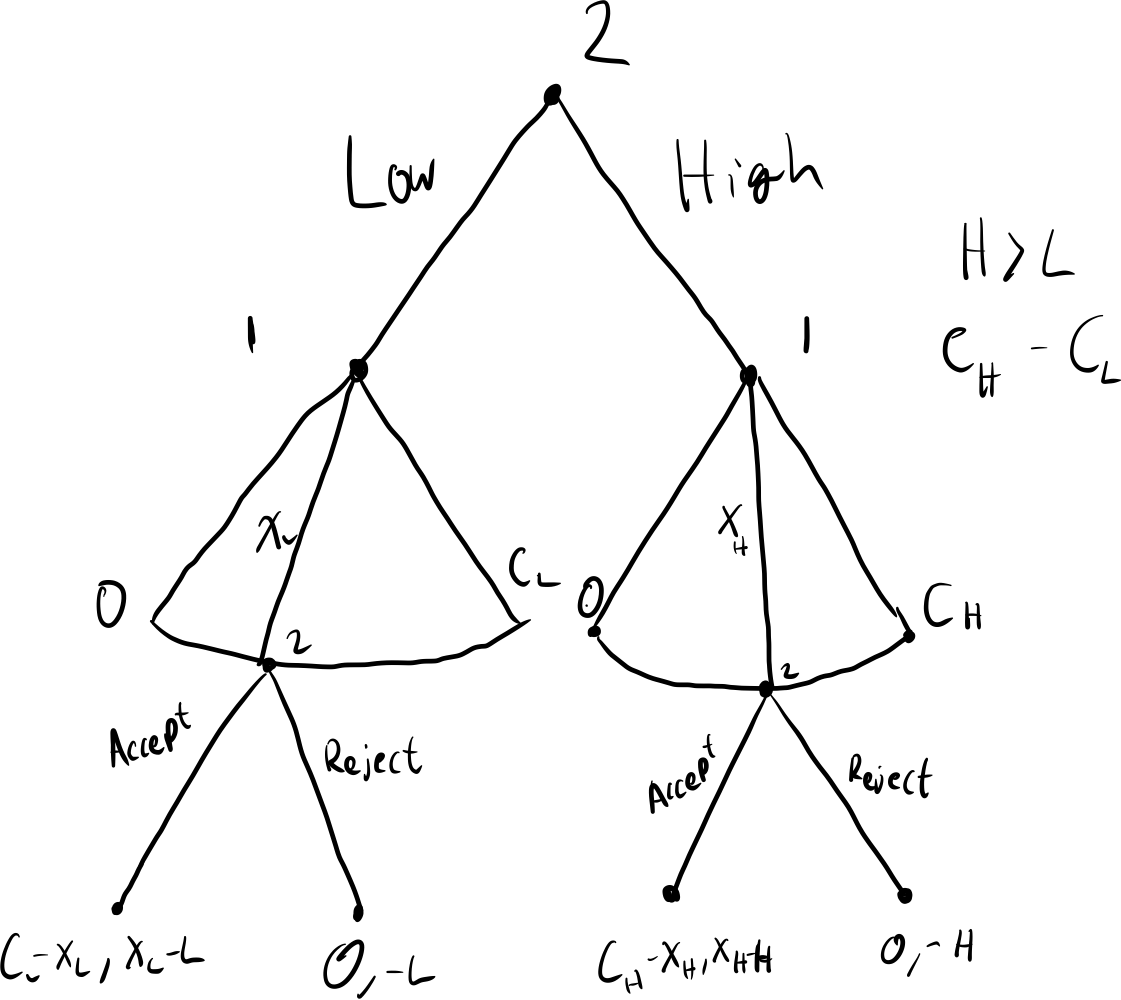
\includegraphics[width=10cm]{images/holdup.png}
      \end{center}
      \tcblower
      We know that in each ultimatum subgame, the subgame perfect equilibrium is
      \begin{align*}
        s_1 &= 0\\
        s_2(x) &= A
      \end{align*}
      If Player 2 plays Low, their payoff in the Low subgame is $-L$, while if Player 2 plays High, their payoff in the High subgame is $-H$.\\

      Therefore, the subgame perfect equilibrium is:
      \begin{align*}
        s_1(E) &= 0,~\forall E\\
        s_2(x) &= (E=L,A),~\forall x
      \end{align*}
    \end{problem}
  \begin{problem}{Variations on the Ultimatum Game}
    \begin{tcbraster}[raster columns = 2,colframe = black!75!white,colback=white]
      \tcbincludepdf{images/activity_9.pdf}
    \end{tcbraster}
  \end{problem}
  \begin{problem}{Critiques of SPE}
    Consider the following extensive form game:
    \begin{center}
      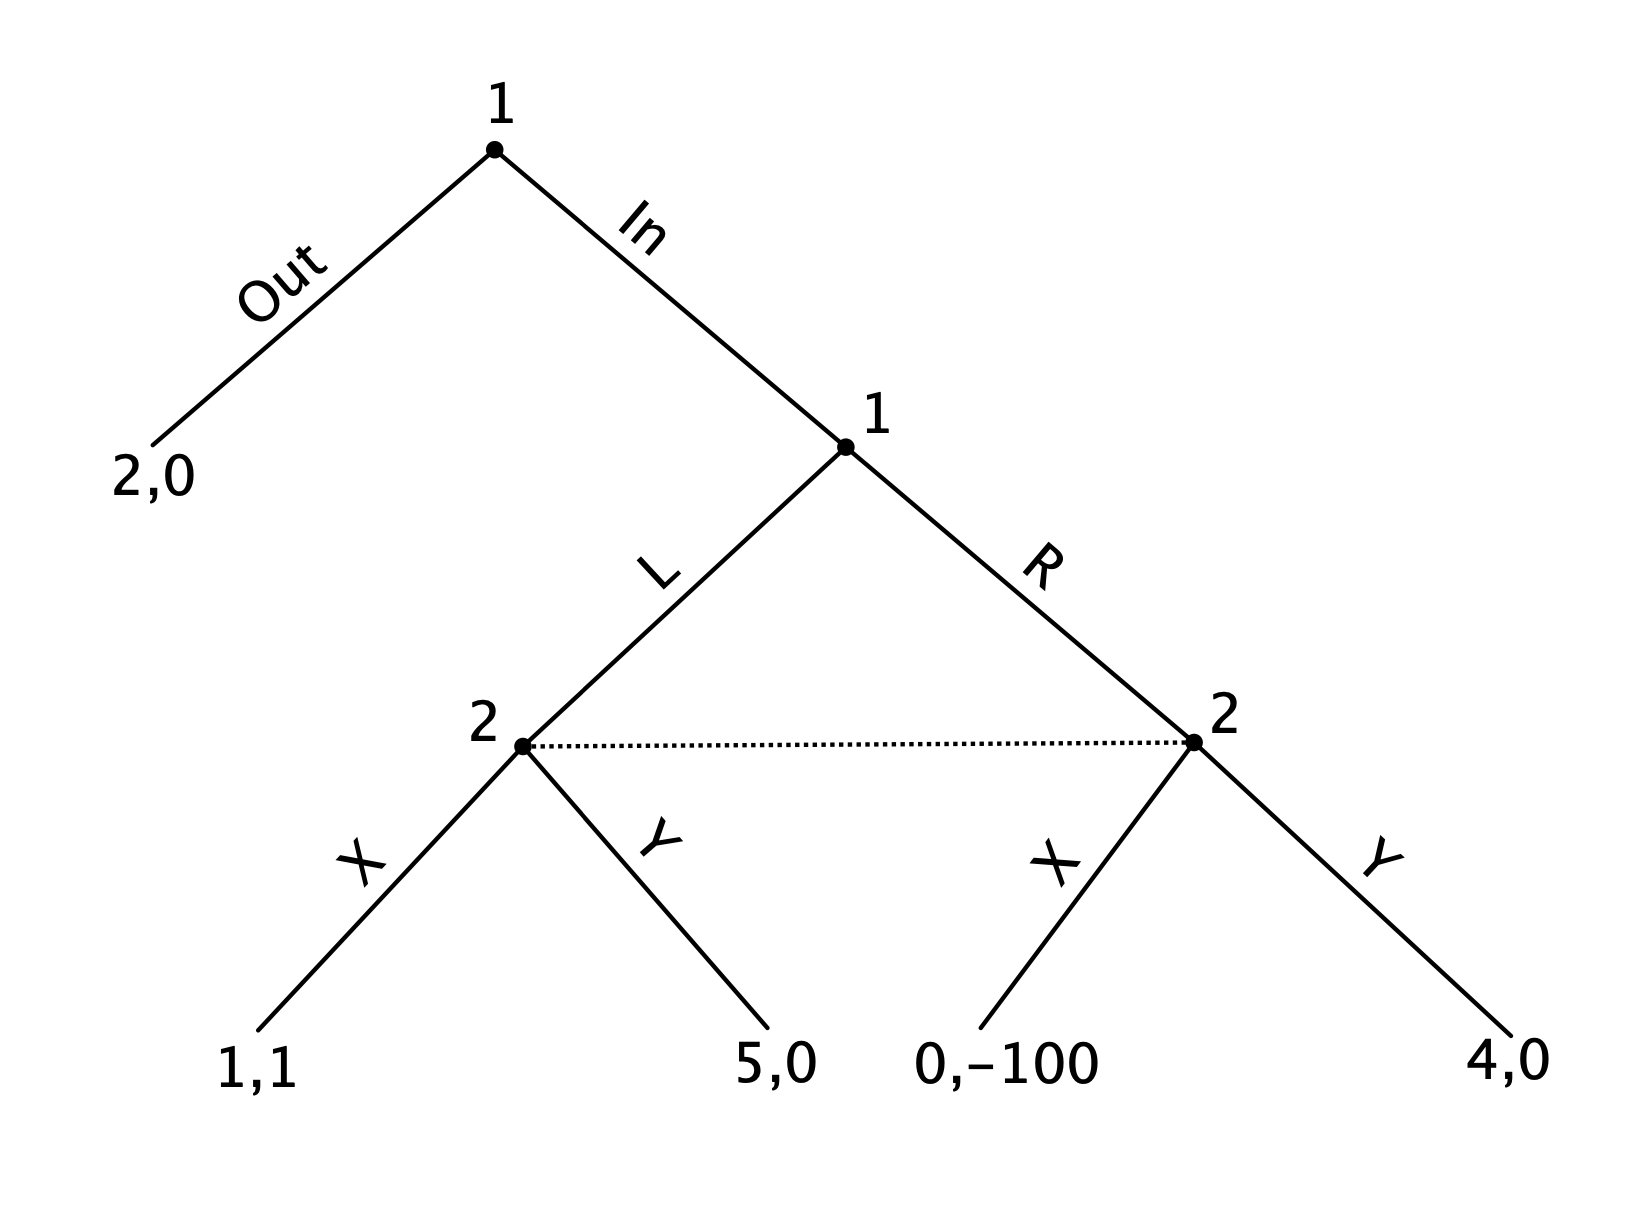
\includegraphics[width=10cm]{images/spe_critique.png}
    \end{center}
    We can see that in the proper subgame, $(L,X)$ is the Nash equilibrium, meaning that player $1$ plays Out, meaning the subgame perfect equilibrium is $(\text{Out},L,X)$.\\

    However, this depends on on Player 2 trusting that player 1 is rational with near 100\% certainty --- if player 1 chooses to play In, then $R$ in the simultaneous-move game, then player 2 has a large negative payoff. Player 2 may want to choose $Y$ if they reason that player $1$ may not be rational.\\

    Similarly, in the centipede game, the SPE is to always play $L$; however, experimental evidence suggests most people play $R$ until close to the end of the game. This is because people either don't backward induct or they reason that their opponent won't backward induct.
    \begin{center}
      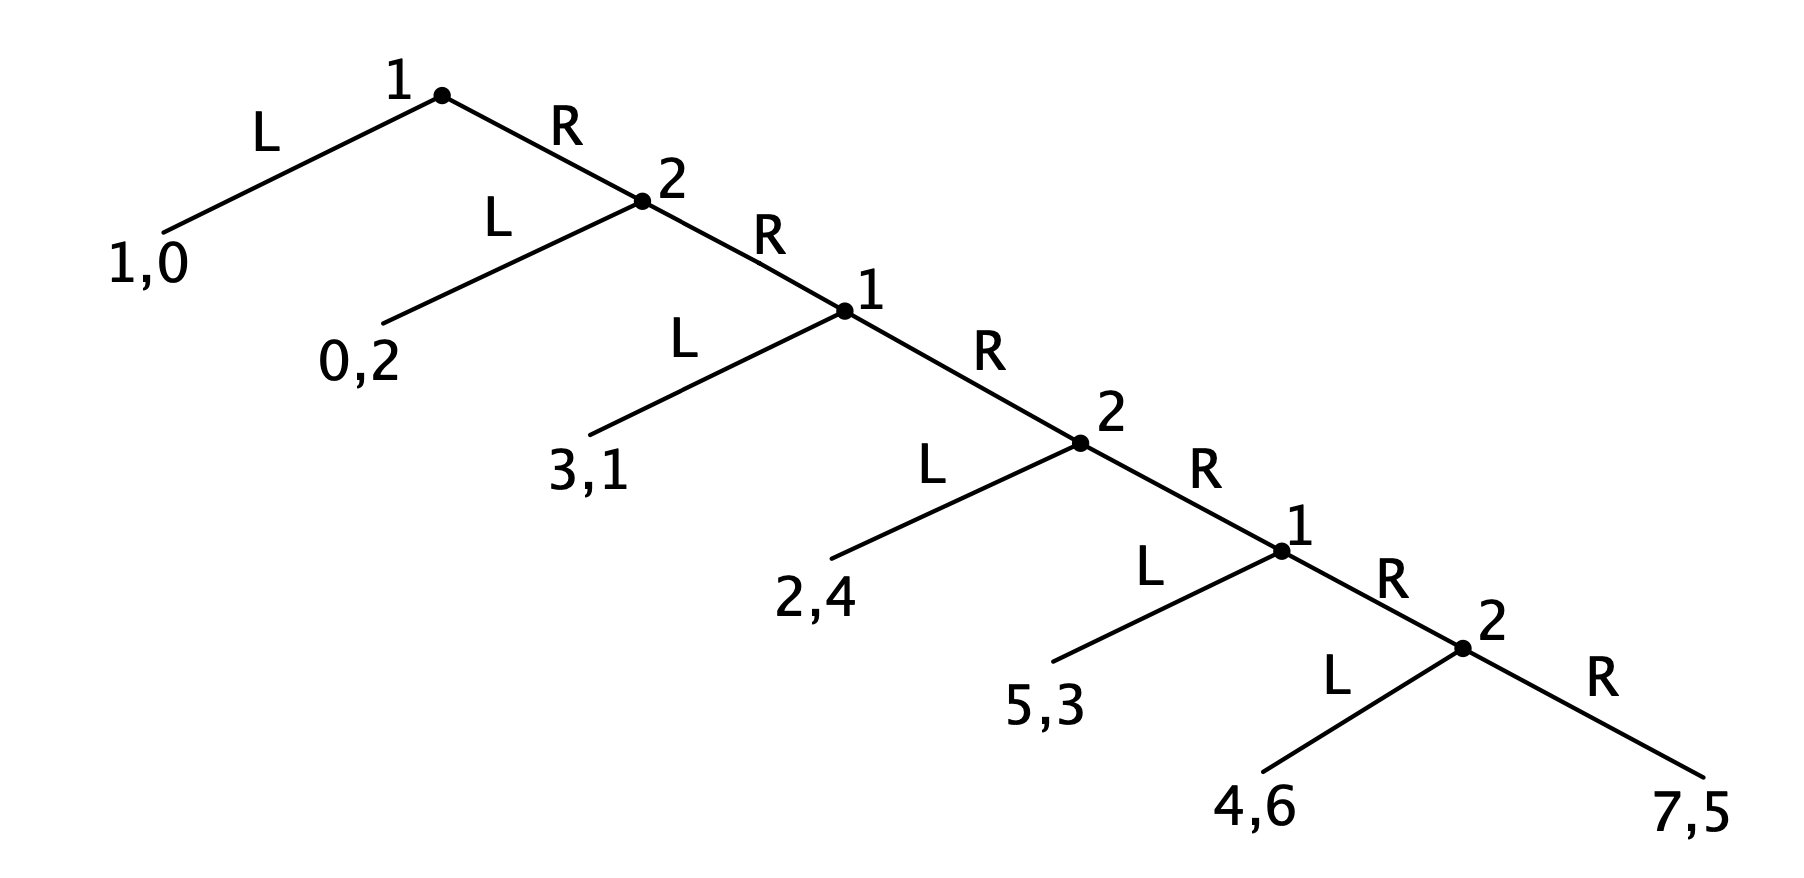
\includegraphics[width=10cm]{images/centipede.png}
    \end{center}
  \end{problem}
  \begin{problem}{Multistage Games}
    \begin{itemize}
      \item A multistage game is a sequence of normal-form stage games.
      \item The stage games are played sequentially by the same players.
      \item Payoffs are received at every stage, not just at the end of the game.
      \item After each stage, the outcome of the previous stage is common knowledge.
    \end{itemize}
    Specifically, we focus on repeated games. We need to be concerned with strategic interactions as players repeatedly play the same game.\\

    For example, in the Prisoner's Dilemma, we can design a repeated game such that $(Q,Q)$ is part of the SPE. More generally, we can create situations in which repeated play allows for cooperation and improvements in total payoff over one-shot play.\\

    Let $G$ be a $n$-player simultaneous move game. The repeated game $G(T,\delta)$ is the game where in periods $t = 1,2,\dots,T$ the players simultaneously choose actions $(a_1^t,a_2^t,\dots,a_n^t)$ after observing all previous actions. We define payoffs in the game by
    \begin{align*}
      v_i\left(s_i,s_{-i}\right) &= \sum_{t=1}^{t}\delta^{t-1}v_i(a_1^t,\dots,a_n^t)
    \end{align*}
    where $(a_1^t,\dots,a_n^t)$ is the action profile taken in period $t$ when players follow strategies $s_1,\dots,s_n$ and $v_i$ are the payoffs for the players in each stage game.\\

    All strategies in the repeated games are complete contingent plans which specify the actiosn that each player will choose after observing all possible previous sequences of actions.\\

    The parameter $\delta\in (0,1]$ denotes the discount factor.
    \begin{itemize}
      \item $\delta$ can be akin to psychological time preferences --- if $\delta$ is low, then players are impatient, while if $\delta$ is high, players are patient.
      \item If we define $\delta = \frac{1}{1+r}$, where $r$ is the interest rate, then $\$100$ in the next period is worth $\$\delta 100$ today since one must invest $\$\delta 100$ into a bank account to get $\$100$ in the next period.
      \item $\delta$ can denote the probability of the end of the game; given that the game reaches stage $t$, the game continues to stage $t+1$ with probaiblity $\delta$ and ends with probability $1-\delta$. The expected number of periods is $\frac{1}{1-\delta}$ is finite.
    \end{itemize}
  \end{problem}
  \begin{problem}{Repeated Games and SPE Activity}
    \begin{tcbraster}[raster columns = 2,colframe = black!75!white,colback=white]
      \tcbincludepdf{images/activity_10.pdf}
    \end{tcbraster}
  \end{problem}
  \begin{problem}{Finitely Repeated Games: Unique Nash Equilibria}
    We find the SPE in a finitely repeated game via backward induction, as we would for a normal extensive-form game.\\

    In the finitely repeated Prisoner's Dilemma has a unique SPE in which each player's \textit{strategy} is to choose $F$ in each period, regardless of the history.\\

    The finite repetition of a stage game $G$ that has a unique Nash equilibrium gives a unique SPE in which players play the Nash equilibrium in every stage, \textit{regardless of what happened prior.}
  \end{problem}
  \begin{problem}{Finitely Repeated Games: Multiple Nash Equilibria}
    Consider the game where the following stage game is repeated twice:
    \begin{center}
      \renewcommand{\arraystretch}{1.5}
      \begin{tabular}{c|c|c|c|}
        \multicolumn{1}{c}{} & \multicolumn{1}{c}{$L$}& \multicolumn{1}{c}{$C$}& \multicolumn{1}{c}{$R$}\\
        \cline{2-4}
        $T$ & $1,1$ & $5,0$ & $0,0$\\
        \cline{2-4}
        $M$ & $0,5$ & $4,4$ & $0,0$\\
        \cline{2-4}
        $B$ & $0,0$ & $0,0$ & $3,3$\\
        \cline{2-4}
      \end{tabular}
    \end{center}
    To solve for the SPE of this game, we have to apply backward induction.\\

    In the second round, a Nash equilibrium must be played, so we start by finding the Nash equilibria of the stage game.
    \begin{itemize}
      \item $M$ is strictly dominated by a combination of $T$ and $B$.
      \item $C$ is strictly dominated by a combination of $L$ and $R$.
    \end{itemize}
    \begin{center}
      \renewcommand{\arraystretch}{1.5}
      \begin{tabular}{c|c|c|c|}
        \multicolumn{1}{c}{} & \multicolumn{1}{c}{$L$}& \multicolumn{1}{c}{$\xcancel{C}$}& \multicolumn{1}{c}{$R$}\\
        \cline{2-4}
        $T$ & $1,1$ & $\xcancel{5,0}$ & $0,0$\\
        \cline{2-4}
        $\xcancel{M}$ & $\xcancel{0,5}$ & $\xcancel{4,4}$ & $\xcancel{0,0}$\\
        \cline{2-4}
        $B$ & $0,0$ & $\xcancel{0,0}$ & $3,3$\\
        \cline{2-4}
      \end{tabular}
    \end{center}
    \begin{itemize}
      \item Therefore, we have three Nash equilibria:
        \begin{itemize}
          \item $(T,L)$ with payoff $(1,1)$
          \item $(B,R)$ with payoff $(3,3)$
          \item $(3/4T + 1/4B,3/4L + 1/4R)$ with payoff $(3/4,3/4)$
        \end{itemize}
      \item Example SPE: play a Nash equilibrium in the stage game in period $1$, and any Nash equilibrium of the stage game in period $2$, regardless of the history.
      \item However, we can also achieve outcomes in the first stage that are not Nash equilibria of the stage game by using the Nash equilibria in the second stage as reward and punishment.
      \item The following is a SPE where $(M,C)$ is played in the first stage:
        \begin{align*}
          (s_1,s_2) &= \begin{cases}
            (M,C) & \text{in stage 1}\\
            (B,R) & \text{in stage 2 if $(M,C)$ in stage 1}\\
            (T,L) & \text{in stage 2 otherwise}
          \end{cases}
        \end{align*}
      \item We can see that this is a SPE as we play a Nash equilibrium in every proper subgame; we can also see that player 1 and player 2 both have no profitable deviation (if player 1 plays $T$ in stage 1, their total payoff is $6$, as compared to $7$ in this strategy profile).
      \item This exhibits the primary function of multiple Nash equilibria in a repeated stage game: using them as rewards and punishments for cooperation/non-cooperation.
    \end{itemize}
  \end{problem}
  \begin{problem}{Finitely Repeated Game}
    \begin{tcbraster}[raster columns = 1,colframe = black!75!white,colback=white]
      \tcbincludepdf{images/activity_11.pdf}
    \end{tcbraster}
  \end{problem}
  \begin{problem}{Infinitely Repeated Stage Games}
    Consider the repeated Prisoner's Dilemma, but infinitely so.
    \begin{itemize}
      \item The argument that the unique SPE of this repeated game was $(F,F)$ was via backward induction.
      \item However, in an infinitely repeated game, we cannot make the argument from backward induction (where is the ``final'' stage game?).
      \item Can we sustain some cooperation in the infinitely repeated game?
    \end{itemize}
  \end{problem}
  \begin{problem}{One Stage Deviation Property}
    A strategy profile in an infinitely repeated game with $\delta < 1$ is a SPE if and only if no player can increase their payoff by changing their action at a single information set, given the other players' strategies and the rest of their own strategy.
    \begin{itemize}
      \item Any profitable deviation can be broken into a sequence of one-period changes --- so, we only need to check single deviations
      \item For infinite horizon games, discounting is crucial to make the theorem true, as it allows payoffs in a far enough future to be worth little.
      \item We assume that all infinite horizon games are such that $\delta < 1$.
    \end{itemize}
    To check whether a strategy profile is a SPE:
    \begin{itemize}
      \item Classify all the information sets on and off the equilibrium path
      \item Apply the One Stage Deviation Property to each class separately
    \end{itemize}
    A strategy in which players play the same Nash Equilibrium of the stage game in each period, \textit{regardless of the history}, is always a SPE.
  \end{problem}
  \begin{problem}{Grim Trigger Strategy}
    The \textit{discounted average} of any stream of payoffs $(v_{i}^{1},v_{i}^{2},\dots)$ for the discount factor $\delta$ is
    \begin{align*}
      (1-\delta)\sum_{t=1}^{\infty}\delta^{t-1}v_{i}^t
    \end{align*}
    If a player received a constant stream of payoffs $(c,c,c,\dots)$, then the discounted average would be $c$.\\
    \vspace{4pt}
    \rule{\textwidth}{0.4pt}
    \vspace{4pt}
    In the Prisoner's Dilemma, define the grim trigger strategy to be
    \begin{align*}
      s_{i}(a^1,\dots,a^t) &= \begin{cases}
        Q&\text{if } (a^1,\dots,a^t) = ((Q,Q),\dots,(Q,Q))\\
        F&\text{otherwise}
      \end{cases}
    \end{align*}
    \begin{description}
      \item[Claim:] The strategy profile in which both players use the grim trigger strategy is a SPE of the infinitely repeated Prisoner's Dilemma for $\delta \geq 1/2$.
    \end{description}
    Suppose there has been a defection at some point in the past to $F$.
    \begin{itemize}
      \item Player $i$'s (current period) average discounted payoff by following the grim trigger: $1$
      \item Player $i$'s average discounted payoff by deviating to $Q$ in the current period, then returning to $s_i$:
        \begin{align*}
          v_i &= (1-\delta)(\overbrace{0}^{\substack{\text{\tiny deviation}\\\text{\tiny payoff}}} + \delta + \delta^2 + \dots) \\
              &= (1-\delta)\left(\sum_{t=1}^{\infty}\delta^t\right)\\
              &= \delta\\
              &< 1
        \end{align*}
    \end{itemize}
    Suppose there has been no defection to $F$ anytime in the past.
    \begin{itemize}
      \item Player $i$'s average discounted payoff by following the grim trigger: $2$ (both players play $(Q,Q)$ at all stages).
      \item Player $i$'s average discounted payoff by deviating to $F$, then following the grim trigger:
        \begin{align*}
          v_i &= (1-\delta)(\overbrace{3}^{\substack{\text{\tiny deviation}\\\text{\tiny payoff}}} + \underbrace{\delta + \delta^2 + \dots}_{\text{\tiny grim trigger for $F$}})\\
              &= (1-\delta) \left(3 + \sum_{t=1}^{\infty}\delta^{t}\right)\\
              &= 3(1-\delta) + \delta\\
              &= 3-2\delta\\
          2 &\geq 3-2\delta \tag*{Nash equilibrium condition}\\
          \delta &\geq \frac{1}{2}
        \end{align*}
    \end{itemize}
  \end{problem}
  \begin{problem}{Grim Trigger Workthrough}
    \begin{tcbraster}[raster columns = 2,colframe = black!75!white,colback=white]
      \tcbincludepdf{images/activity_12.pdf}
    \end{tcbraster}
  \end{problem}
  \begin{problem}{Rubinstein's Bargaining Game}
    Consider a game in which \$1 is to be divided between two players:
    \begin{itemize}\itemsep -2pt
      \item In periods $1,3,5,\dots$, player $1$ offers the division $(x_1,x_2)$. Player 2 either accepts the offer and the game ends, or rejects the offer and play continues
      \item In periods $2,4,6,\dots$, player $2$ offers the division $(y_1,y_2)$. Player 1 either accepts the offer and the game ends, or rejects the offer and play continues
    \end{itemize}
    If the division $(z,1-z)$ is agreed upon in period $t$, then the payoffs are $(v_1,v_2) = \left(\delta^{t-1}z,\delta^{t-1}(1-z)\right)$.
    \begin{itemize}\itemsep -2pt
      \item Waiting to divide is costly
      \item This game is \textit{infinite} horizon
      \item The game is not repeated
    \end{itemize}
  \end{problem}
  \begin{problem}{SPE of Rubinstein's Bargaining Game}
    \begin{description}
      \item[Proposition] The bargaining game has a unique SPE: in each period the player who proposes offer $\frac{1}{1+\delta}$ to themselves and the other player accepts any division giving them at least $\frac{\delta}{1 + \delta}$, and rejects any offer giving them less.
      \item[Proof of Existence] We want to show that the One Stage Deviation Property is satisfied by the proposed SPE.\\

        There are two types of information sets: when the proposer makes an offer, and when the recipient makes a decision.
        \begin{align*}
          \shortintertext{Proposer payoff from following:}
          v_{p} &= \frac{1}{1+\delta}\\
          \shortintertext{Proposer payoff from deviation:}
          v_{p} &= \delta\frac{\delta}{1+\delta} \tag*{accept following period offer}\\
                &< \frac{1}{1+\delta}\\
                \\
          \shortintertext{Recipient payoff from accepting an offer of $z$ in the current period:}
          v_{r} &= z\\
          \shortintertext{Recipient payoff from rejecting the offer:}
          v_{r} &= \delta\frac{1}{1+\delta} \tag*{provide offer of $\frac{1}{1+\delta}$ in following period}\\
          \shortintertext{Therefore, recipient should accept offer of $z$ if and only if}
          z &\geq \delta\frac{1}{1+\delta}
        \end{align*}
    \end{description}
    \vspace{4pt}
    \rule{\textwidth}{0.4pt}
    \vspace{4pt}
    \begin{description}
      \item[Efficiency:] On the equilibrium path, bargaining is immediate and therefore efficient.
      \item[Patience:] Player $1$ can earn a greater share of the pie if $\delta$ is small (players are impatient)
      \item[First-Mover Advantage:] For all $\delta < 1$, player $1$ earns more than player $2$ in the SPE.
    \end{description}
  \end{problem}
  \begin{problem}{Proving a Bargaining Game SPE}
    Assume the current period.
    \begin{description}
      \item[Proposer Payoffs:]
        \begin{enumerate}[(a)]
          \item Find payoff from following.
          \item Find payoff from offering less, assuming the next period proposer's strategy holds constant.
        \end{enumerate}
      \item[Recipient Payoffs:]
        \begin{enumerate}[(a)]
          \item Find payoff from \textit{accepting the proposer's offer} {\tiny \textbf{Note:} the recipient does not ``deviate'', as they are not in charge of making the proposal.}
          \item Find payoff from \textit{rejecting the proposer's offer}, holding fixed the next period strategy (the current recipient becomes the proposer in the following period).
        \end{enumerate}
    \end{description}
  \end{problem}
  \begin{problem}{Bargaining Workthrough}
    \begin{tcbraster}[raster columns = 1,colframe = black!75!white,colback=white]
      \tcbincludepdf{images/activity_13.pdf}
    \end{tcbraster}
  \end{problem}
  \begin{problem}{Bargaining Extensions and the Folk Theorem}
    Recall the Grim Trigger strategy for the infinitely repeated Prisoner's Dilemma is SPE with $\delta \geq \frac{1}{2}$.\\

    However, this doesn't mean sufficiently patient players will always cooperate in repeated interactions. There are many possible SPE with $\delta \geq \frac{1}{2}$.
    \begin{enumerate}[(a)]
      \item Play $F$ in every period
      \item For $\delta \geq \frac{1}{2}$, there is a SPE in which players play $F$ in the first period and $Q$ in all future periods.
      \item For $\delta \geq \frac{1}{\sqrt{2}}$, there is a SPE in which players play $F$ in every even period and $Q$ in every odd period.
      \item For $\delta \geq \frac{1}{2}$, there is a SPE where the players play $(Q,F)$ in every even period and $(F,Q)$ in every odd period.
      \item For $\delta = 1/2$, there is a SPE where the players play the last-used action of the opponent.
    \end{enumerate}
    \vspace{4pt}
    \rule{\textwidth}{0.4pt}
    \vspace{4pt}
    We would like to characterize what is possible in SPE of infinitely repeated games.
    \begin{itemize}
      \item A payoff vector $v = (v_1,v_2,\dots,v_n)$ is \textit{feasible} if it is a weighted average of the payoffs available in a strategic game.
      \item A payoff vector is \textit{strictly individually rational} if each player obtains strictly more than their min-max payoff.
      \item The min-max payoff is the payoff a player can guarantee themself even if the other players try to punish them as badly as they can.
    \end{itemize}
    \textbf{Folk Theorem:} Suppose that the set of feasible payoffs of $G$ is $n$-dimensional. Then, for any feasible and strictly individually rational payoff vector $v$, $\exists \overline{\delta} < 1$ such that $\forall \delta > \overline{\delta}$, $G(\infty,\delta)$ has a SPE with discount average payoffs $v$.
  \end{problem}
  \begin{problem}{Folk Theorem for Prisoner's Dilemma}
    \begin{center}
      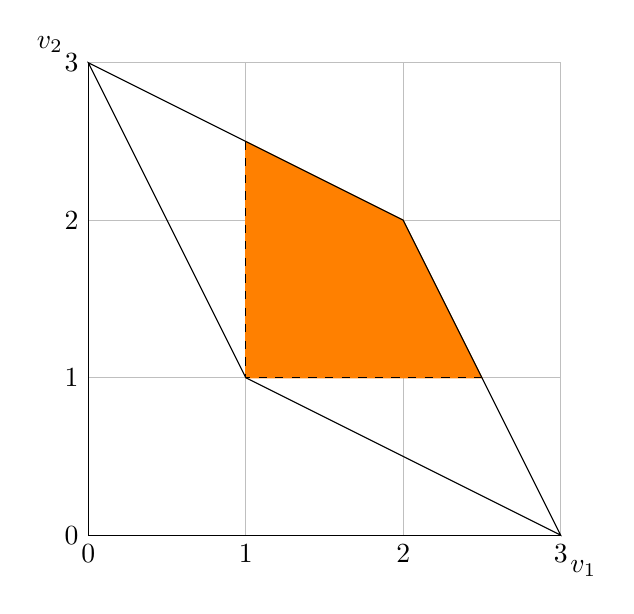
\begin{tikzpicture}[scale=2]
        \draw[color=black!25!white] (0,0) grid (3,3);
        \filldraw[draw = black, color=orange] (1,1) -- (1,2.5) -- (2,2) -- (2.5,1) -- cycle;
        \draw (0,3) -- (0,0) -- (3,0);
        \node[anchor = east] at (0,0) {$0$};
        \node[anchor = east] at (0,1) {$1$};
        \node[anchor = east] at (0,2) {$2$};
        \node[anchor = east] at (0,3) {$3$};
        \node[anchor = north] at (0,0) {$0$};
        \node[anchor = north] at (1,0) {$1$};
        \node[anchor = north] at (2,0) {$2$};
        \node[anchor = north] at (3,0) {$3$};
        \node[anchor = south east] at (-0.1,3) {$v_2$};
        \node[anchor = north west] at (3,-0.1) {$v_1$};
        \draw (0,3) -- (2,2) -- (3,0) -- (1,1) -- cycle;
        \draw[dashed] (1,2.5) -- (1,1) -- (2.5,1);
      \end{tikzpicture}
    \end{center}
    The feasible payoffs are defined by the outer diamond --- the min-max payoff for each player is $1$, since the worst punishment a rival can inflict is to choose $F$.
  \end{problem}
  \begin{problem}{Folk Theorem for Bach or Stravinsky}
    \begin{center}
      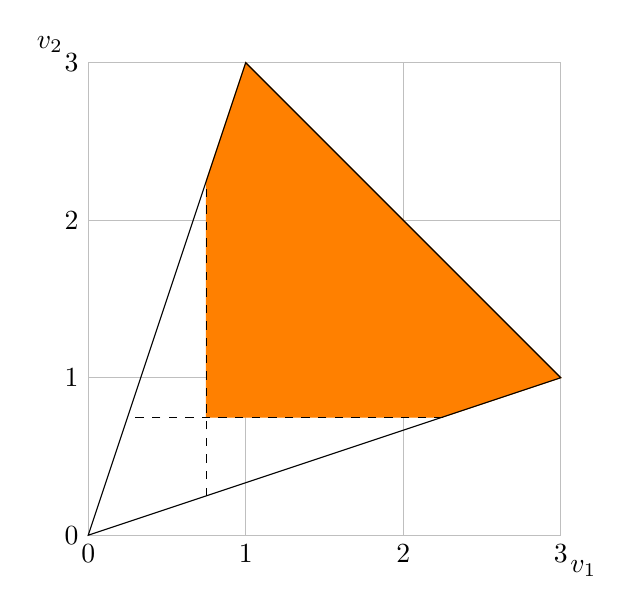
\begin{tikzpicture}[scale = 2]
        \draw[color=black!25!white] (0,0) grid (3,3);
        \filldraw[color=orange] (0.75,0.75) -- (0.75,2.25) -- (1,3) -- (3,1) -- (2.25,0.75) -- cycle;
        \draw (0,0) -- (1,3) -- (3,1) -- cycle;
        \node[anchor = east] at (0,0) {$0$};
        \node[anchor = east] at (0,1) {$1$};
        \node[anchor = east] at (0,2) {$2$};
        \node[anchor = east] at (0,3) {$3$};
        \node[anchor = north] at (0,0) {$0$};
        \node[anchor = north] at (1,0) {$1$};
        \node[anchor = north] at (2,0) {$2$};
        \node[anchor = north] at (3,0) {$3$};
        \node[anchor = south east] at (-0.1,3) {$v_2$};
        \node[anchor = north west] at (3,-0.1) {$v_1$};
        \draw[dashed] (0.75,0.25) -- (0.75,2.25);
        \draw[dashed] (2.25,0.75) -- (0.25,0.75);
      \end{tikzpicture}
    \end{center}
    The feasible payoffs are the triangle bounded by the outer triangle --- the min-max payoff for each player is $3/4$ since the worst punishment a rival can inflict is to choose $\frac{1}{4}B + \frac{3}{4}S$
  \end{problem}
  \section*{Games of Incomplete Information}%
  \begin{problem}{Narrowing the Scope}
    In real life economic situation, it's unlikely that players know:
    \begin{itemize}
      \item payoffs
      \item who other players are
      \item what moves are possible
      \item how outcomes depend on actions
      \item what players know
    \end{itemize}
    We will focus on the case where the players know who the other players are, and their available actions, but not how those actions impact payoffs. These are known as \textit{Bayesian Games}.
  \end{problem}
  \begin{problem}{Example I: Public Goods Game}
    \begin{center}
      \begin{tabular}{c|c|c|}
        \multicolumn{1}{c}{} & \multicolumn{1}{c}{Clean} & \multicolumn{1}{c}{Don't}\\
        \cline{2-3}
        Clean & $1-c_1,1-c_2$ & $1-c_1$,1\\
        \cline{2-3}
        Don't & $1,1-c_2$ & $0,0$
      \end{tabular}
    \end{center}
    Assume that the actions are chosen simultaneously and that players don't know their own costs.
    \begin{description}
      \item[(I.a):] Player $2$ also knows player $1$'s cost, but player $1$ believes that $c_2 \in \{\underline{c},\overline{c}\}$ where $\underline{c}< \overline{c}$, and the low cost is true with probability $p$.
      \item[(I.b):] Each player believes that the cost of the other roommate is equally likely to be any value between $0$ and $2$: $c_1,c_2 \sim U[0,2]$
    \end{description}
  \end{problem}
  \begin{problem}{Example II: Auction}
    Consider a two-bidder \textbf{first-price sealed bid private value auction}:
    \begin{itemize}
      \item Sealed bid: announce $b_1$ and $b_2$ simultaneously
      \item First-price: the highest bidder wins and pays their bid
      \item Private value: valuation of the object, $\theta_i$, is independent of how others view the object
      \item A coin is flipped if they choose the same bid
    \end{itemize}
    In this case, utilities are:
    \begin{align*}
      v_i(b_i,b_{-i}) &= \begin{cases}
        \theta_i - b_i & b_i > b_{-i}\\
        \frac{1}{2}(\theta_i-b_i) & b_i = b_{-i}\\
        0 & b_i < b_{-i}
      \end{cases}
    \end{align*}
    The primary form of incomplete information here is that each player knows their own valuation, but does not know their rival's --- assume each player believes that the valuation of the rival is uniform on $[0,1]$
  \end{problem}
  \begin{problem}{Characterization of Bayesian Games}
    A static game with incomplete information $G$ consists of
    \begin{itemize}
      \item A set of types $\Theta_i$ for each player $i$. Player $i$'s type is privately known to player $i$.
      \item A set of actions $A_i$ for each player $i$.
      \item A joint probability distribution $\phi(\theta_1,\dots,\theta_n)$
      \item A payoff function $v_i(a_1,\dots,a_n;\theta_1,\dots,\theta_n)$ for each player $i$
    \end{itemize}
    This information is common knowledge.\\

    For example, in our examples, we had the type spaces:
    \begin{description}
      \item[(I.a):] $\Theta_1 = \{c_1\}$, $\Theta_2 = \{\underline{c},\overline{c}\}$
      \item[(I.b):] $\Theta_1=\Theta_2 = [0,2]$
      \item[(II):] $\Theta_1 = \Theta_2 = [0,1]$
    \end{description}
    The payoffs depend on the action profile and the types of all players.
  \end{problem}
  \begin{problem}{Harsanyi's Observation and Bayesian Pure Strategy}
    Games of incomplete information can be thought of as games of complete but imperfect information wher eNature is another player who moves first. Not everyone is informed about Nature's move --- Nature chooses $\theta \in \Theta$ with probability $\phi(\theta)$, but only tells $\theta_i$ to player $i$.\\

    Harsanyi's observation makes it possible to define strategies and equilibria just the same way we defined them in extensive form games. A strategy is (still) a function that assigns an action to each information set for each player.
    \begin{itemize}
      \item A \textit{Bayesian pure strategy} is a function that assigns an action for each possible type. $s_i: \Theta_i \rightarrow A_i$
    \end{itemize}
  \end{problem}
\end{document}
